% ============================================================
% DataBattle 2026 — EDA & Feature Engineering Report
% ============================================================
\documentclass[12pt,a4paper]{article}

\usepackage[margin=2.5cm, headheight=15pt]{geometry}
\usepackage{amsmath,amssymb}
\usepackage{graphicx}
\usepackage{booktabs}
\usepackage{longtable}
\usepackage{array}
\usepackage{xcolor}
\usepackage{hyperref}
\usepackage{caption}
\usepackage{subcaption}
\usepackage{float}
\usepackage{enumitem}
\usepackage{titlesec}
\usepackage{parskip}
\usepackage{fancyhdr}
\usepackage{multirow}

% ── Colors ──────────────────────────────────────────────────
\definecolor{truecolor}{HTML}{E74C3C}
\definecolor{falsecolor}{HTML}{3498DB}
\definecolor{accentcolor}{HTML}{2C3E50}
\definecolor{goldcolor}{HTML}{F39C12}
\definecolor{greencolor}{HTML}{27AE60}

% ── Header / Footer ─────────────────────────────────────────
\pagestyle{fancy}
\fancyhf{}
\rhead{DataBattle 2026}
\lhead{EDA \& Feature Engineering Report}
\rfoot{\thepage}

% ── Title ───────────────────────────────────────────────────
\title{
  \vspace{-1cm}
  {\Large \textbf{DataBattle 2026}}\\[0.4em]
  {\large Exploratory Data Analysis \& Feature Engineering Report}\\[0.3em]
  {\normalsize Predicting the Last Cloud-to-Ground Lightning Strike at French Airports}
}
\author{%
  \textbf{Team:} Solveit \\[0.4em]
  Weldegebriel Tesfay Hagos \quad Fisha Mehabaw Alemayoh
}
\date{March 2026}

% ============================================================
\begin{document}
\maketitle
\thispagestyle{fancy}

\tableofcontents
\newpage

% ============================================================
\section{Executive Summary}
% ============================================================

This report documents the complete exploratory data analysis (EDA) and feature engineering
pipeline for the DataBattle 2026 competition. The task is binary classification:
given a cloud-to-ground (CG) lightning strike near a French airport during a storm alert,
predict whether it is the \textbf{last} CG strike of that storm event.

\subsection*{Key Findings at a Glance}

\begin{itemize}[leftmargin=1.5em]
  \item \textbf{2,627 storm segments} across 5 French airports (Ajaccio, Bastia, Biarritz, Nantes, Pise)
  \item \textbf{Severe class imbalance}: 4.6\% True (last strike) vs. 95.4\% False
  \item \textbf{Rule baseline}: F1 = 0.9885, AUC = 0.9994 — sets a very high bar for ML
  \item \textbf{Strongest signal}: time gap before a strike (\texttt{time\_since\_prev}, $|r|=0.216$)
  \item \textbf{41 features engineered} across 11 physical groups covering amplitude, silence,
        position, rolling activity, outer-ring context, and temporal patterns
  \item \textbf{Critical insight}: the outer ring (20--50 km) collapses 8.8$\times$ before the
        last strike — a powerful context signal
\end{itemize}

% ============================================================
\section{Dataset Structure}
% ============================================================

\subsection{Data Partitions}

The raw dataset contains lightning strikes near five French airports.
After pre-processing it splits into three functional DataFrames:

\begin{table}[H]
\centering
\caption{Dataset partitions}
\begin{tabular}{llr}
\toprule
\textbf{Partition} & \textbf{Description} & \textbf{Rows} \\
\midrule
\texttt{df\_cg}      & CG strikes inside 20 km zone (model input) & 56,599 \\
\texttt{df\_inside}  & All strikes inside 20 km (includes IC)      & $>$56,599 \\
\texttt{df\_outside} & All strikes outside 20 km (context only)   & $\approx$450,472 \\
\bottomrule
\end{tabular}
\end{table}

\noindent The model is trained only on \texttt{df\_cg}.
In-cloud (IC) strikes (\texttt{icloud=True}) are excluded because they carry no target label.
Outside-zone strikes are used purely as context features for the outer-ring feature (Group K).

\subsection{Segment Definition}

A \emph{segment} is the fundamental unit of prediction: all CG strikes from a single
storm event at a single airport. Segments are identified by:

\begin{equation}
  \texttt{segment\_key} = \texttt{airport} \;+\; \text{``\_''} \;+\; \texttt{airport\_alert\_id}
\end{equation}

\noindent Verified property: \textbf{exactly one} \texttt{is\_last\_lightning\_cloud\_ground = True}
per segment, across all 2,627 segments.

\subsubsection*{Confirmed Variable Structure}

\begin{itemize}[leftmargin=1.5em]
  \item \texttt{airport\_alert\_id}: populated for \textbf{all 56,599 inside-zone rows}
        (within the 20 km alert zone). \texttt{NaN} only for the 450,472 outside-zone rows —
        not missing in the modelling sense. Acts as a per-airport sequential alert counter.
        The segment key is \texttt{airport + alert\_id}.
  \item \texttt{is\_last\_lightning\_cloud\_ground}: boolean, populated for all inside-zone rows.
        \texttt{True} = last CG strike before a 30-minute silence window.
        Exactly \textbf{one True per segment}: 2,627 True / 53,972 False.
\end{itemize}

\noindent\textbf{Open question (pending Meteorage):} whether the 450,472 outside-zone rows
should be used for model training via a constructed \texttt{remaining\_time} target
(see Section~\ref{sec:target_construction}).

\begin{figure}[H]
  \centering
  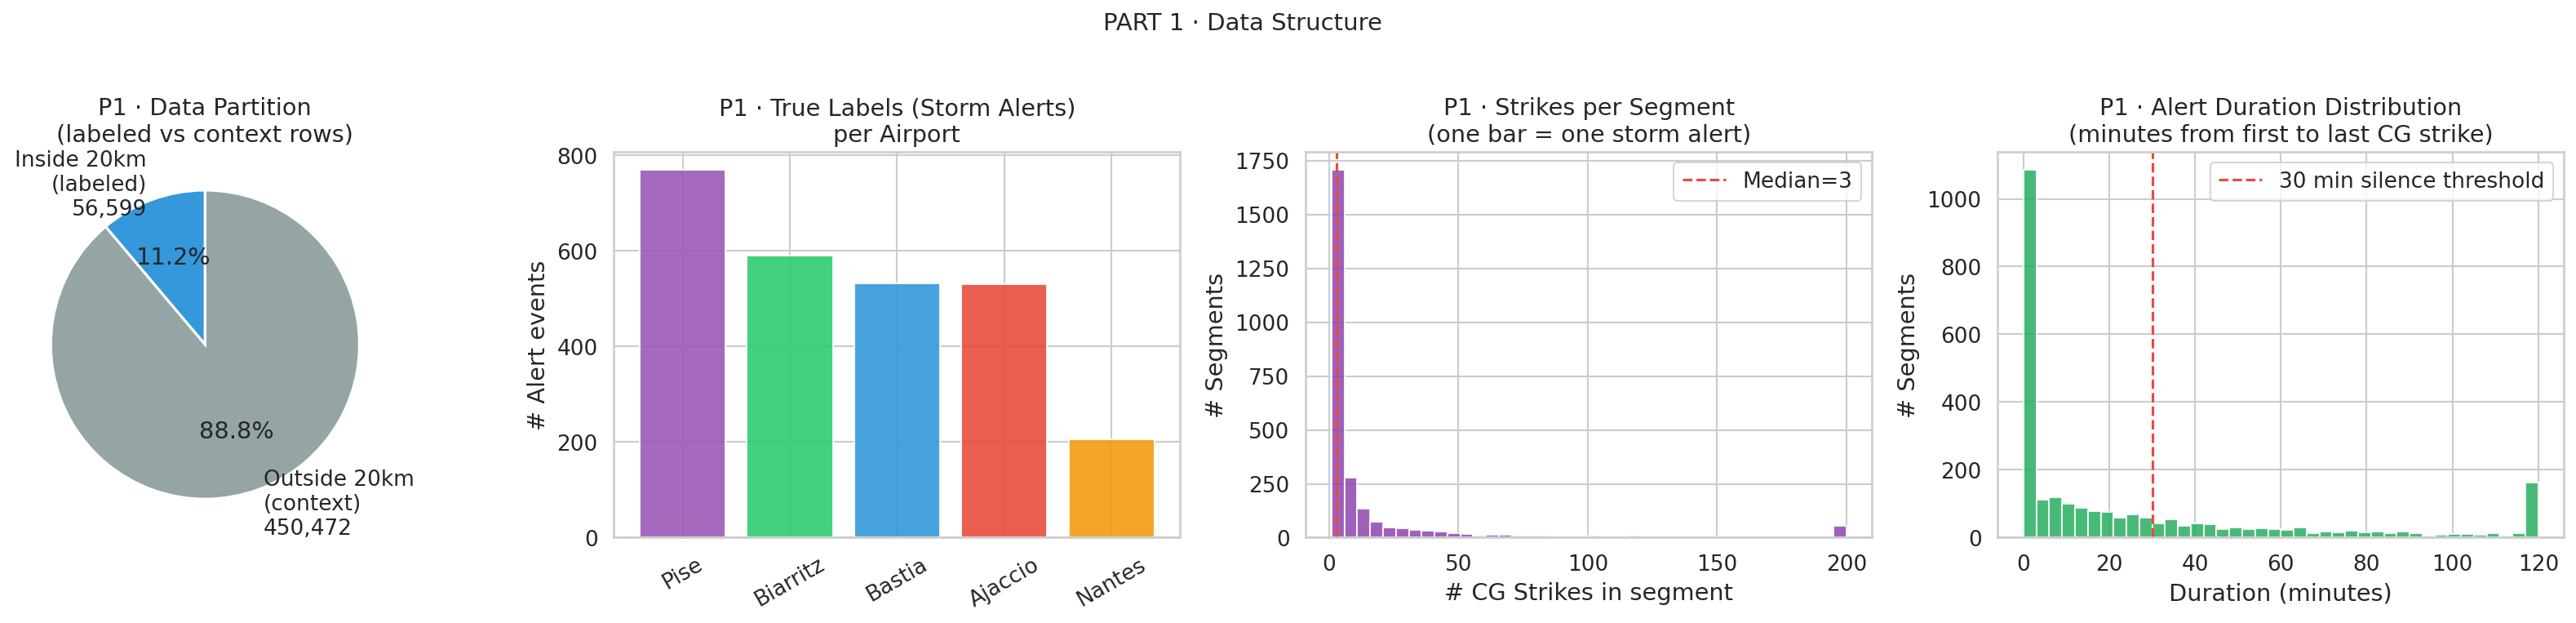
\includegraphics[width=0.92\textwidth]{figures/p1_data_structure.png}
  \caption{Data structure verification — 1 True label per segment, segment size distributions}
  \label{fig:data_structure}
\end{figure}

\subsection{Single-Row Segments}

\textbf{945 segments} contain exactly one CG strike. By definition that strike is
simultaneously the first and last, so its target is always True. These segments require
\emph{sentinel fill values} for all lag/delta features (no previous strike exists):

\begin{table}[H]
\centering
\caption{Sentinel fill values for single-row segments}
\begin{tabular}{lrl}
\toprule
\textbf{Feature} & \textbf{Fill} & \textbf{Rationale} \\
\midrule
\texttt{time\_since\_prev}    & 99,999 & No previous strike — treat as infinite silence \\
\texttt{dist\_delta}          & 0      & No movement information — neutral \\
\texttt{amp\_delta}           & 0      & No change information — neutral \\
\texttt{cg\_count\_Nmin}      & 1      & Only 1 strike known in any window \\
\texttt{rolling\_mean\_mag}   & median & Population median as neutral reference \\
\bottomrule
\end{tabular}
\end{table}

% ============================================================
\section{Target Analysis}
% ============================================================

\subsection{Class Imbalance}

\begin{table}[H]
\centering
\caption{Target class distribution}
\begin{tabular}{lrrl}
\toprule
\textbf{Class} & \textbf{Count} & \textbf{Share} & \textbf{Meaning} \\
\midrule
\textcolor{truecolor}{\textbf{True}}  & 2,627  & 4.6\%  & Last CG strike of the storm \\
\textcolor{falsecolor}{\textbf{False}} & 53,972 & 95.4\% & Any other CG strike \\
\midrule
Total & 56,599 & 100\% & \\
\bottomrule
\end{tabular}
\end{table}

\noindent Imbalance ratio is $\approx 1\!:\!20$.
Accuracy is not a meaningful metric (predicting always-False gives 95.4\% accuracy trivially).
Recommended metrics: \textbf{F1-score}, \textbf{AUC-ROC}, \textbf{Brier Score}.
LightGBM configuration: \texttt{scale\_pos\_weight = 20}.

\begin{figure}[H]
  \centering
  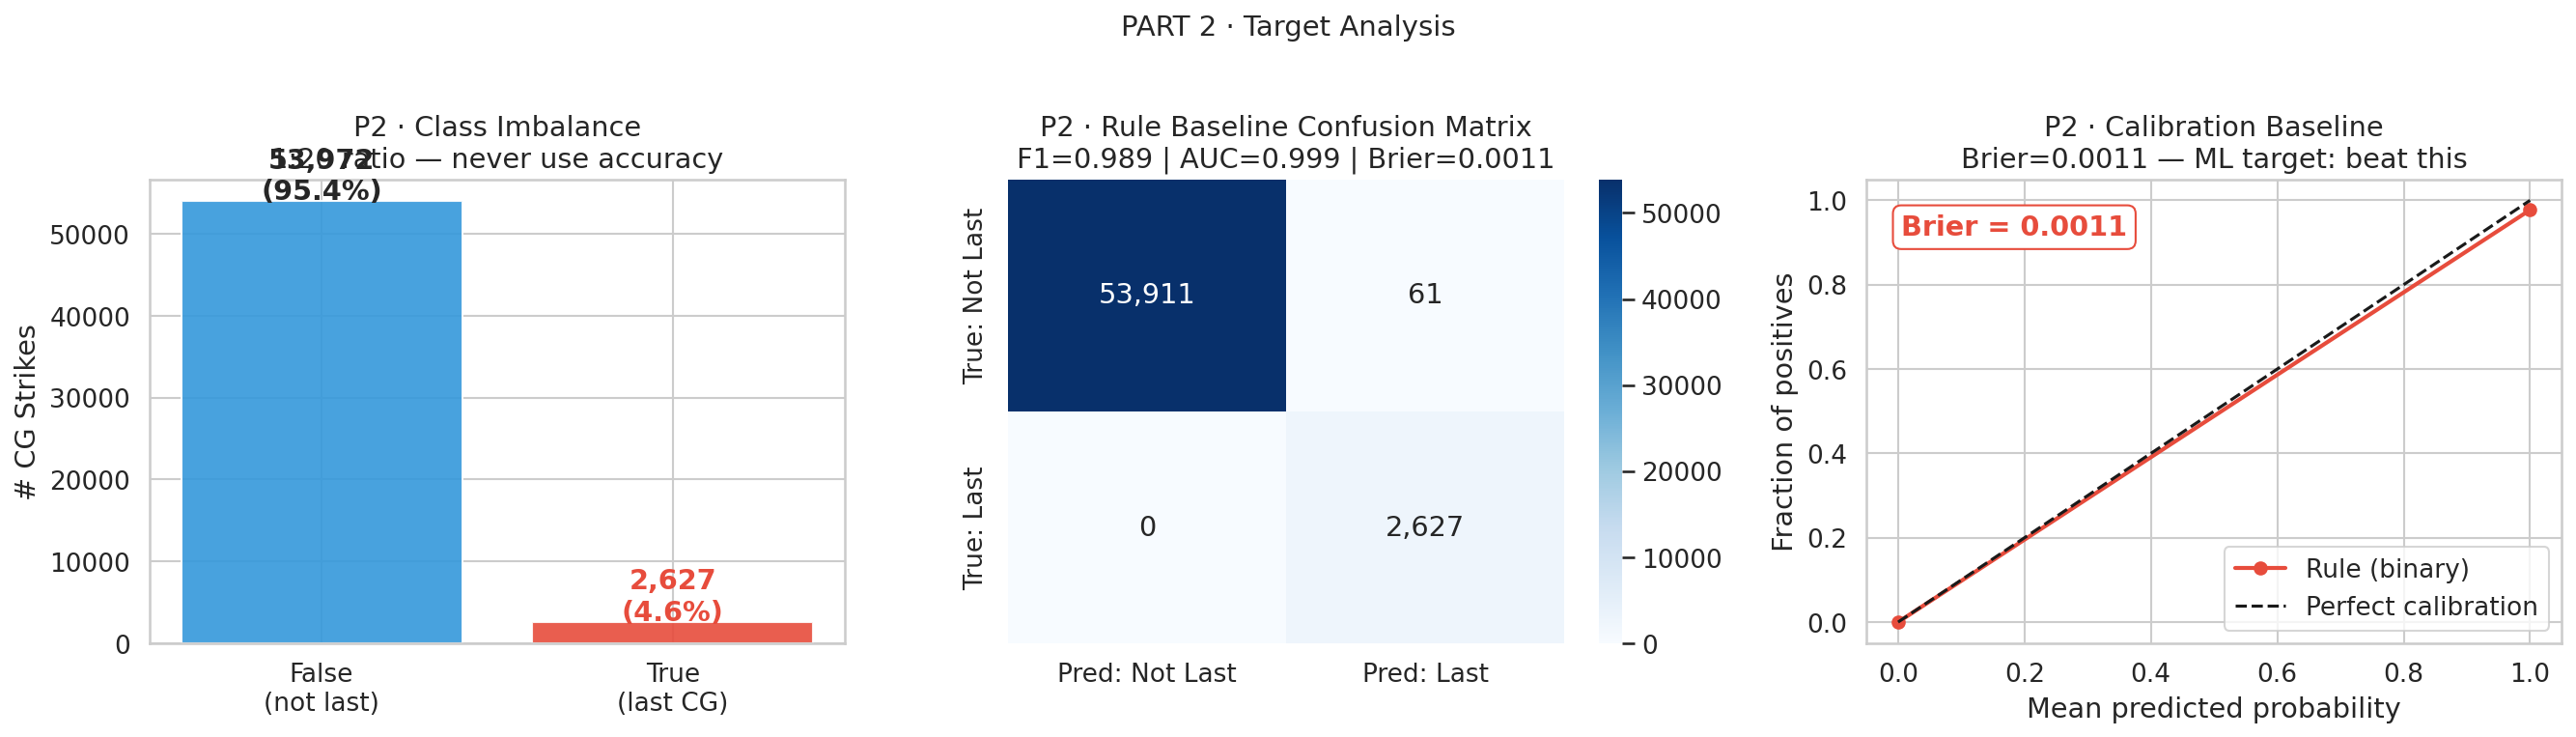
\includegraphics[width=0.92\textwidth]{figures/p2_target_analysis.png}
  \caption{Target distribution and class imbalance visualisation}
  \label{fig:target}
\end{figure}

\subsection{Rule Baseline}

Before any ML, a simple rule baseline is established:
\emph{the last CG strike chronologically in each segment is predicted as True.}

\begin{table}[H]
\centering
\caption{Rule baseline performance}
\begin{tabular}{lr}
\toprule
\textbf{Metric} & \textbf{Value} \\
\midrule
F1-Score      & 0.9885 \\
AUC-ROC       & 0.9994 \\
Brier Score   & 0.0011 \\
Precision     & 0.9773 \\
Recall        & 1.0000 \\
\bottomrule
\end{tabular}
\end{table}

\noindent This near-perfect baseline reflects a fundamental property of the data: the
``last CG'' rule is almost always correct by construction. Any ML model must beat
these values to provide genuine uplift. The challenge is precision: identifying
\emph{which} strike is last \emph{before} it becomes last.

% ============================================================
\subsection{Target Construction for Outside-Zone Rows}
\label{sec:target_construction}
% ============================================================

\noindent\textbf{Note:} The dataset already provides \texttt{is\_last\_lightning\_cloud\_ground}
as a validated binary target for all 56,599 inside-zone CG strikes.
This subsection describes an \emph{alternative} continuous target constructed for the
450,472 outside-zone rows, which carry no provided label.
The two targets serve different purposes:

\begin{table}[H]
\centering
\caption{Primary vs.\ secondary target summary}
\begin{tabular}{lll}
\toprule
\textbf{Target} & \textbf{Scope} & \textbf{Purpose} \\
\midrule
\texttt{is\_last\_lightning\_cloud\_ground} (True/False)
  & 56,599 inside-zone rows & Primary classification target — already provided \\
$y_t = f(\texttt{remaining\_time})$
  & 450,472 outside-zone rows & Secondary target for semi-supervised pretraining \\
\bottomrule
\end{tabular}
\end{table}

\noindent The secondary target is constructed from the time remaining until the storm ends.
A naive linear transform contains a mathematical inconsistency: at the last strike,
\texttt{remaining\_time} $= 30$ min (not 0, due to the 30-minute silence definition).
The corrected transform is:

\begin{align}
  \texttt{remaining\_time\_adj} &= \texttt{remaining\_time} - 30\,\text{min} \\
  y_t &= 1 - \frac{\texttt{remaining\_time\_adj}}{\max(\texttt{remaining\_time\_adj})}
\end{align}

\noindent This ensures $y_t = 1.0$ at the last strike and $y_t = 0.0$ at the first strike.
Use of the outside-zone rows for training is \textbf{pending approval from Meteorage}.

% ============================================================
\section{Raw Feature Signal Analysis}
% ============================================================

\subsection{Amplitude — The Primary Decay Signal}

Amplitude (in kA, with sign) is the most physically meaningful raw feature.
Negative amplitude is the normal polarity of mature storm CG strikes.
\textbf{Positive amplitude signals storm decay}.

\begin{table}[H]
\centering
\caption{Amplitude statistics by class}
\begin{tabular}{lrrl}
\toprule
\textbf{Metric} & \textbf{True strikes} & \textbf{False strikes} & \textbf{Ratio} \\
\midrule
Positive amplitude (\%) & 27.4 & 16.2 & \textbf{1.69$\times$} \\
Negative amplitude (\%) & 72.3 & 83.8 & 0.86$\times$ \\
Mean amplitude (kA)     & $-$8.28 & $-$12.04 & — \\
Mean $|$amplitude$|$ (kA) & 32.38 & 22.32 & 1.45$\times$ \\
\bottomrule
\end{tabular}
\end{table}

\noindent True strikes are 1.69$\times$ more likely to be positive-polarity.
This is the strongest single raw signal in the dataset.

\begin{figure}[H]
  \centering
  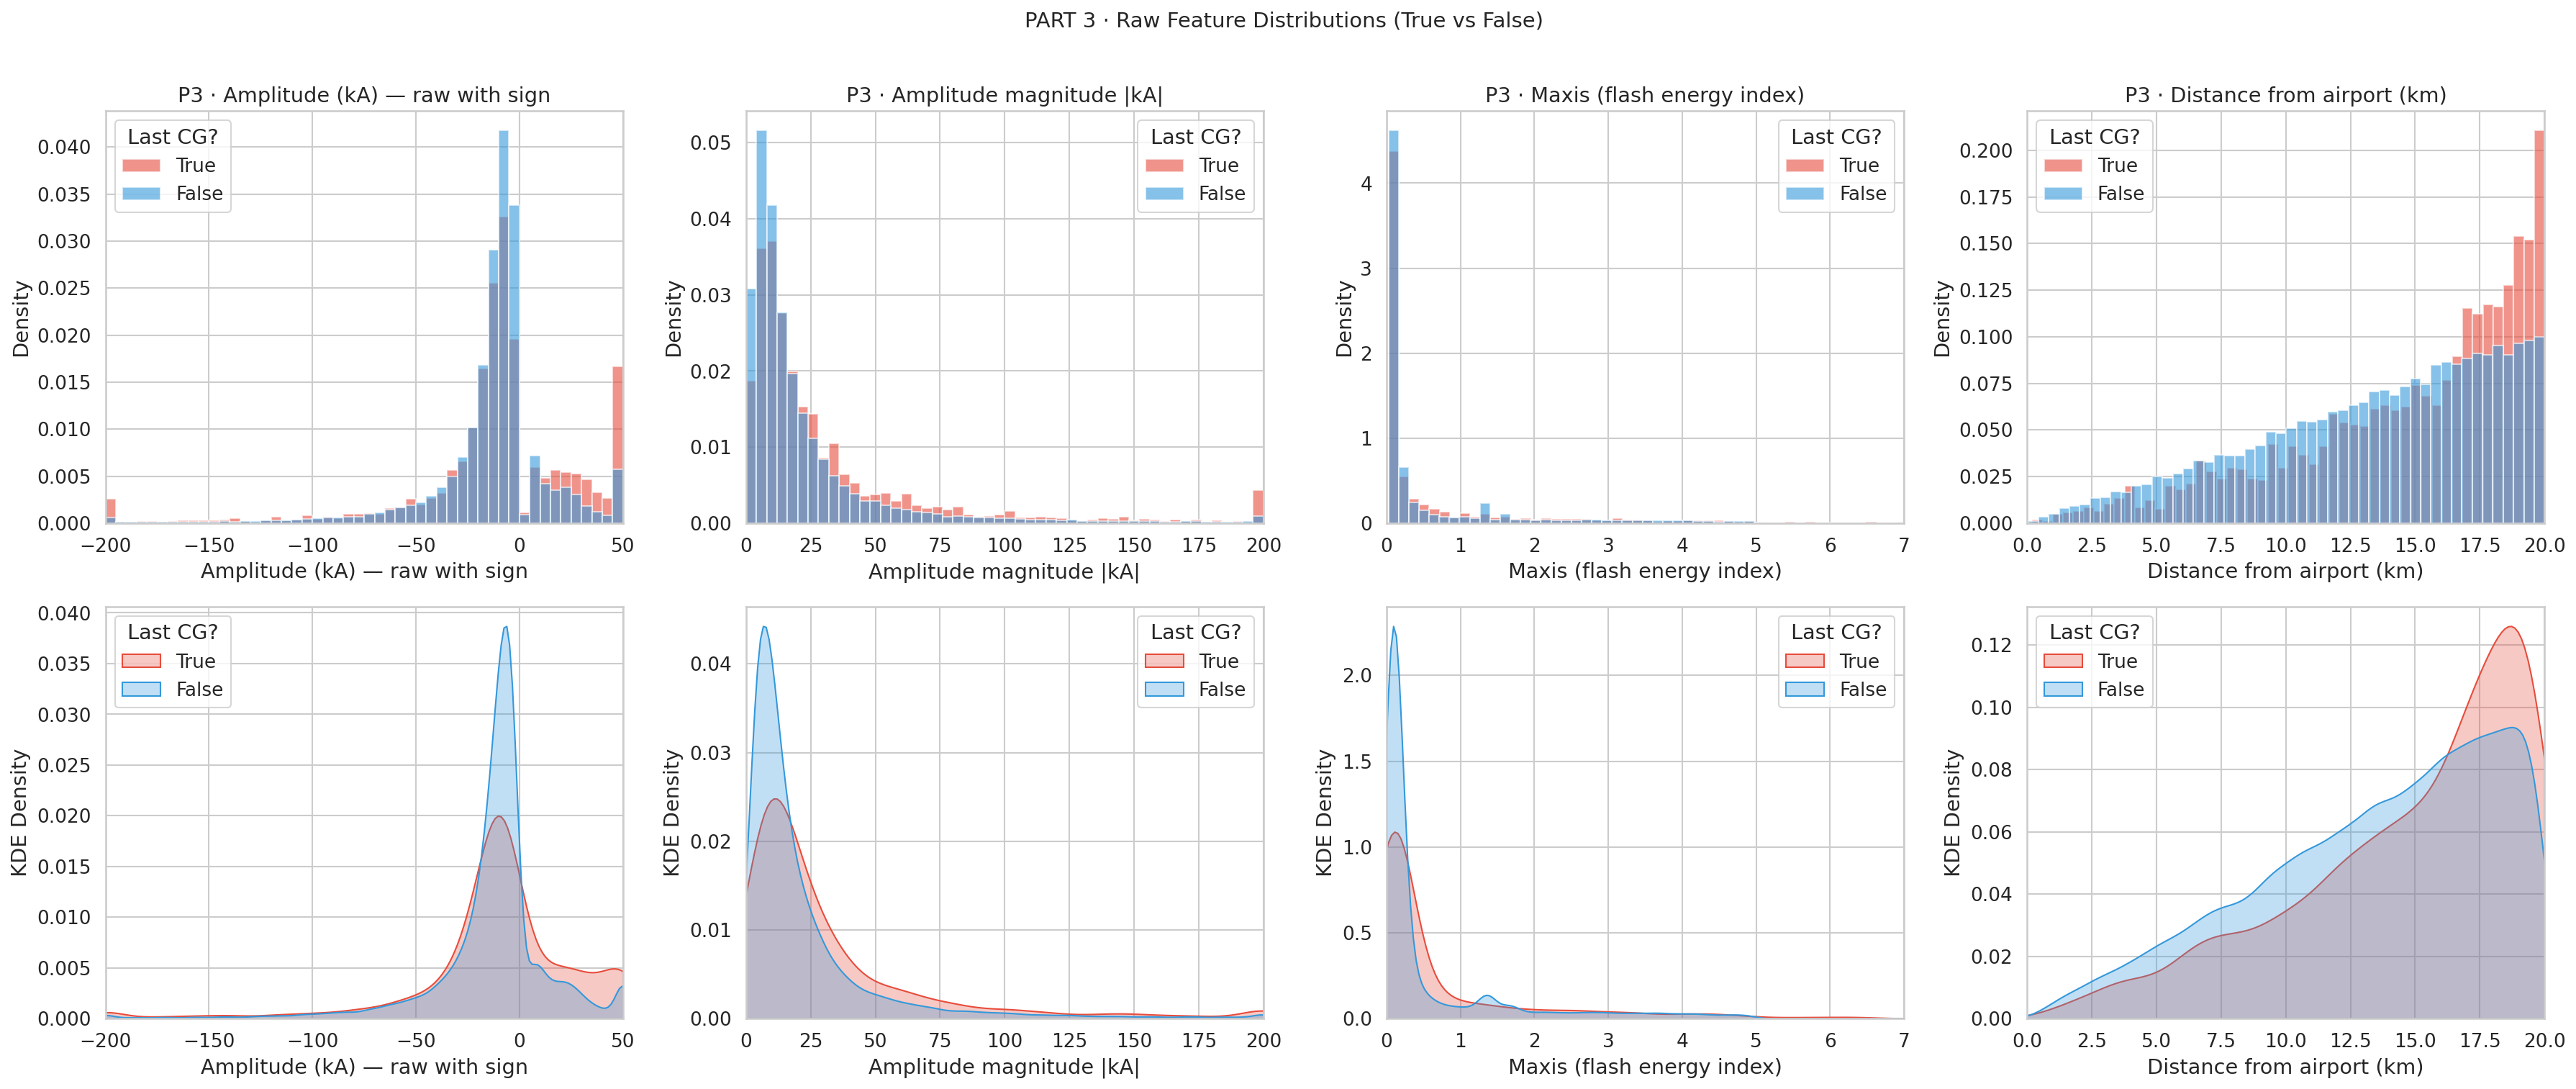
\includegraphics[width=\textwidth]{figures/p3_raw_feature_distributions.png}
  \caption{Raw feature distributions: True vs. False by amplitude, maxis, distance}
  \label{fig:raw_features}
\end{figure}

\subsection{Other Raw Features}

\begin{table}[H]
\centering
\caption{Raw feature signal assessment}
\begin{tabular}{llp{7cm}}
\toprule
\textbf{Feature} & \textbf{Signal} & \textbf{Finding} \\
\midrule
\texttt{amplitude} (sign)   & Strong  & Positive polarity 1.69$\times$ more common in True \\
\texttt{amp\_magnitude}     & Moderate & True strikes larger magnitude ($|$32 vs. 22 kA$|$) \\
\texttt{dist}               & Weak    & Slight tendency for True strikes to be further away \\
\texttt{maxis}              & Weak    & Flash energy weakly correlated with target \\
\texttt{azimuth}            & None    & Storms approach from all directions equally \\
\texttt{strike\_x/y}        & Weak    & Coordinate position less useful than distance \\
\bottomrule
\end{tabular}
\end{table}

% ============================================================
\section{Storm Lifecycle Analysis}
% ============================================================

\subsection{The Biarritz Case Study}

Segment \texttt{Biarritz\_1.0} contains 11 CG strikes with 1 True label.
It illustrates the canonical storm decay pattern:

\begin{enumerate}[leftmargin=1.5em]
  \item \textbf{Early phase}: high-frequency negative-polarity strikes, close approach
  \item \textbf{Middle phase}: strikes begin to thin out, polarity shifts toward positive
  \item \textbf{Decay phase}: long silence ($>$15 min), positive polarity dominant
  \item \textbf{Last strike (True)}: occurs after the longest gap, highest positive-polarity
        probability, storm moving away from airport
\end{enumerate}

\begin{figure}[H]
  \centering
  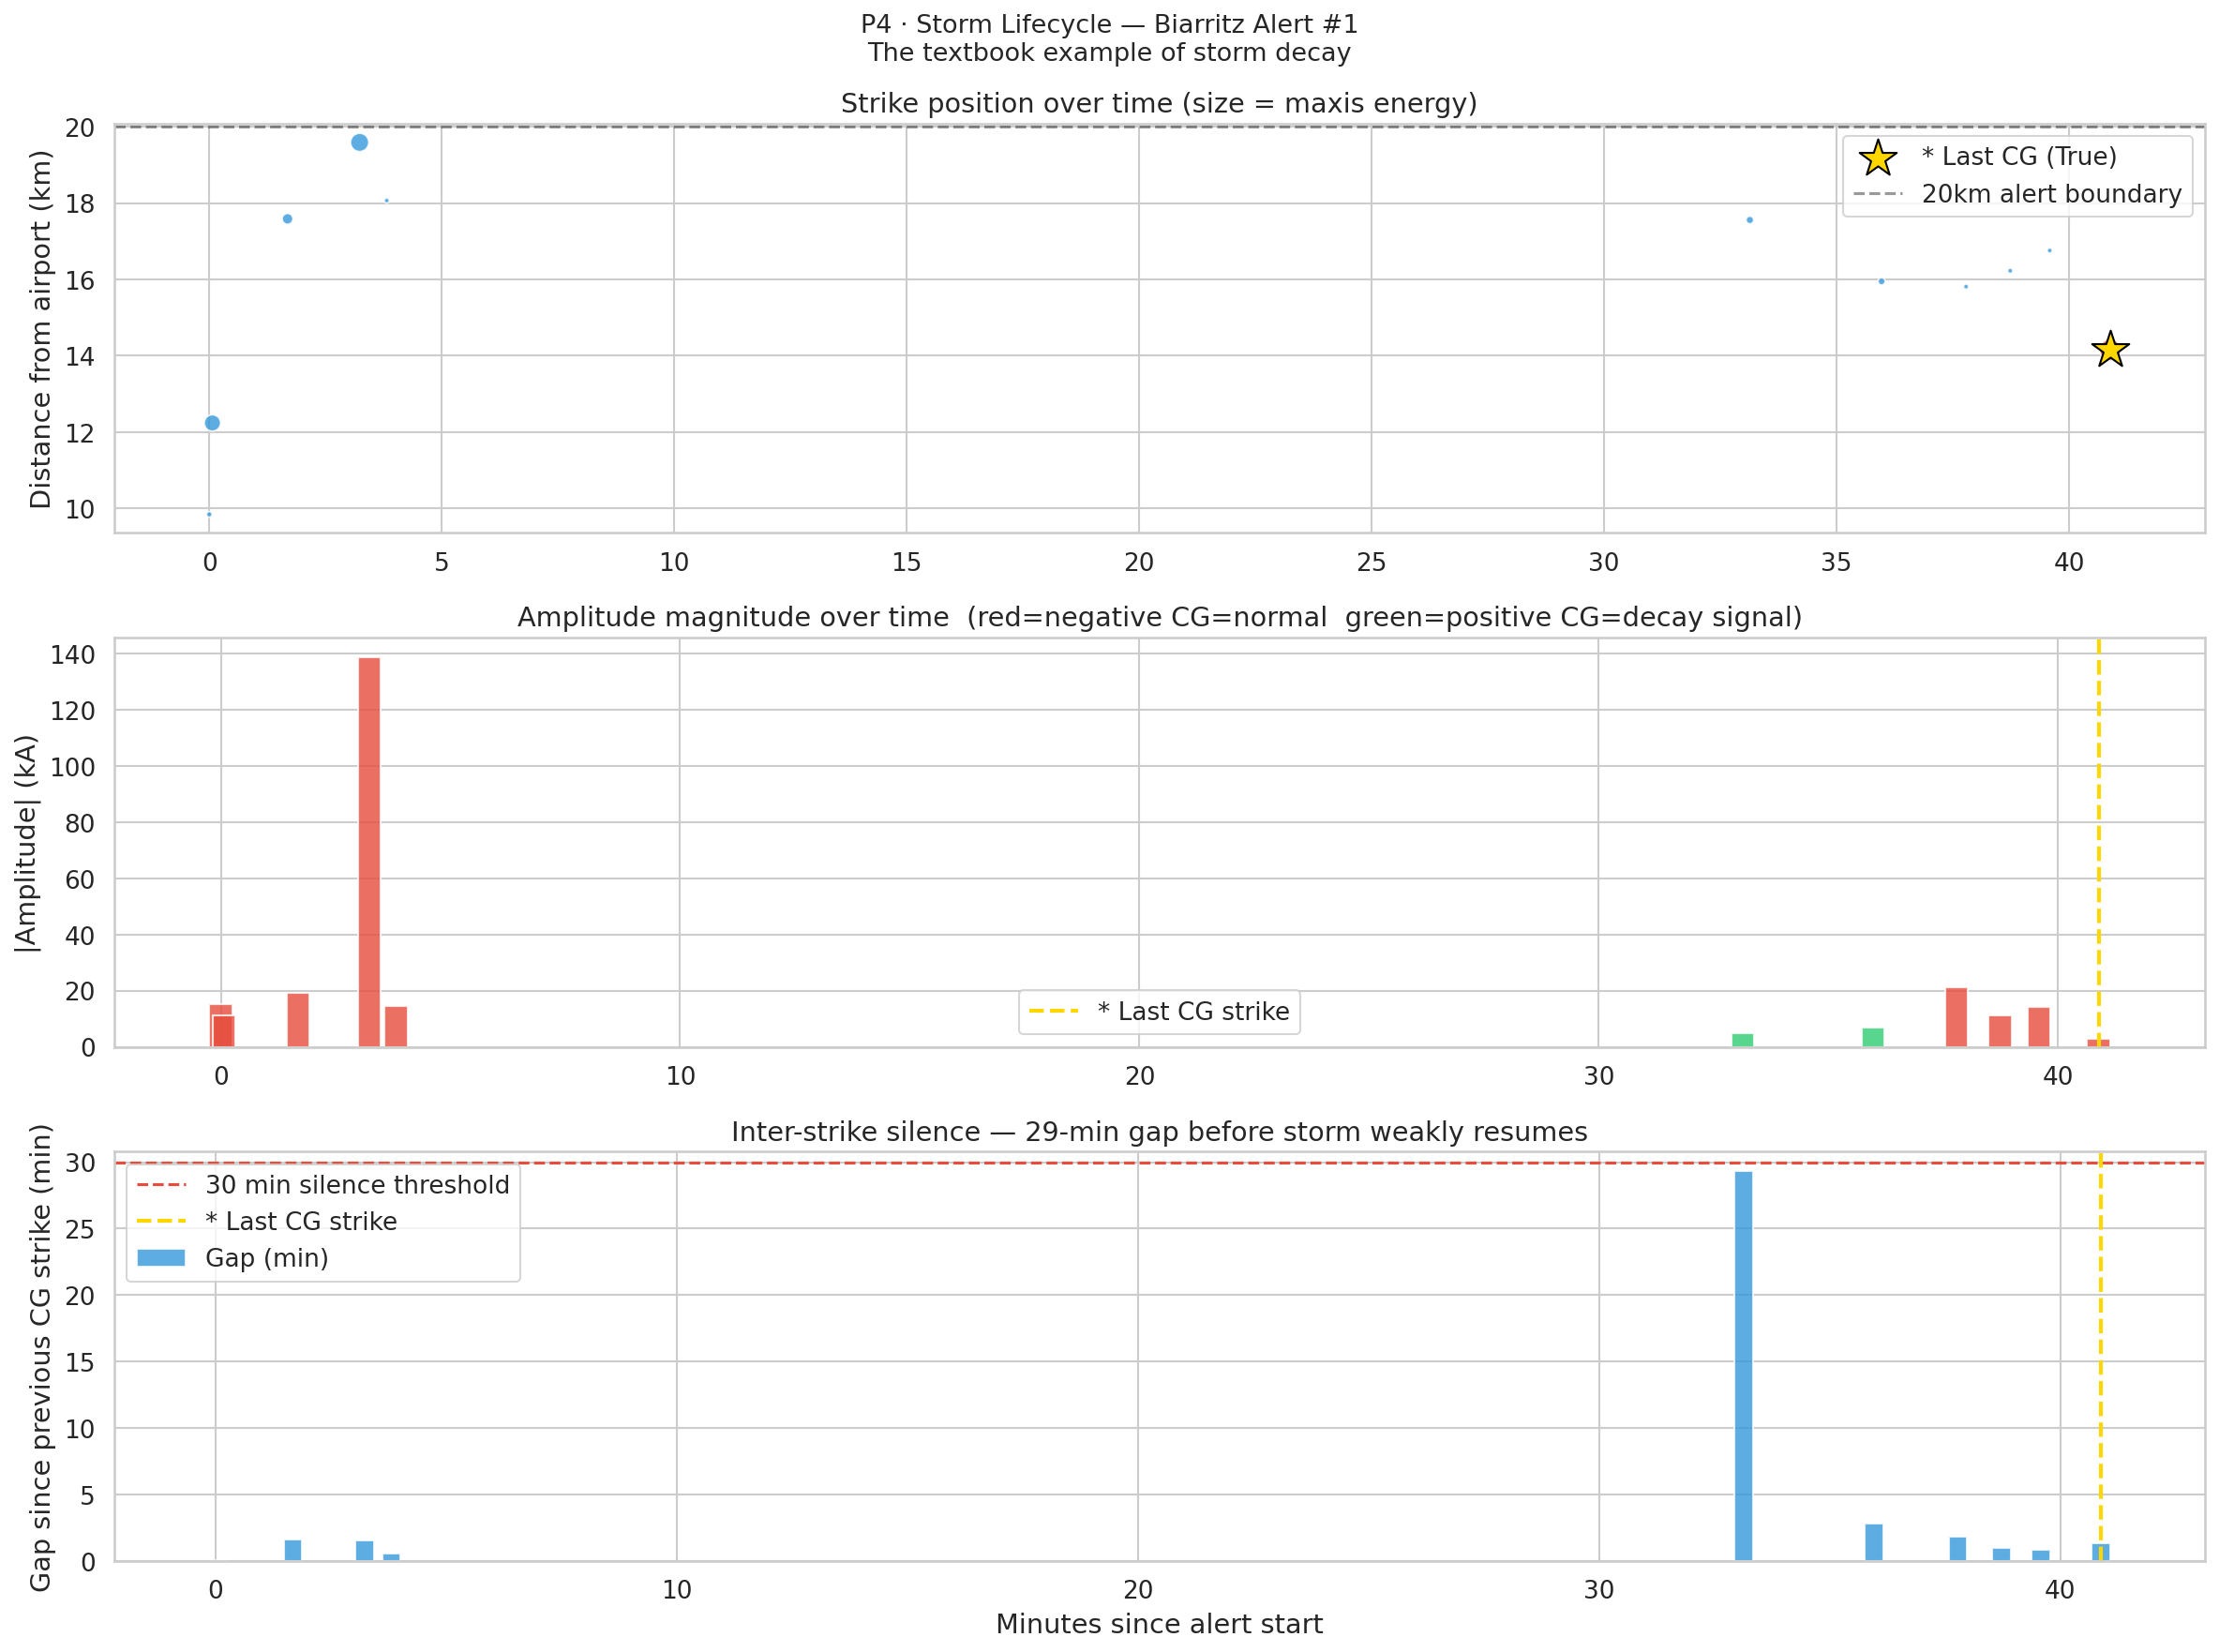
\includegraphics[width=\textwidth]{figures/p4_biarritz_storm_lifecycle.png}
  \caption{Biarritz storm lifecycle: distance, amplitude, and inter-strike gaps over time.
           Gold marker = last CG strike (True label).}
  \label{fig:biarritz}
\end{figure}

\subsection{Decay Pattern Across All Storms}

\begin{figure}[H]
  \centering
  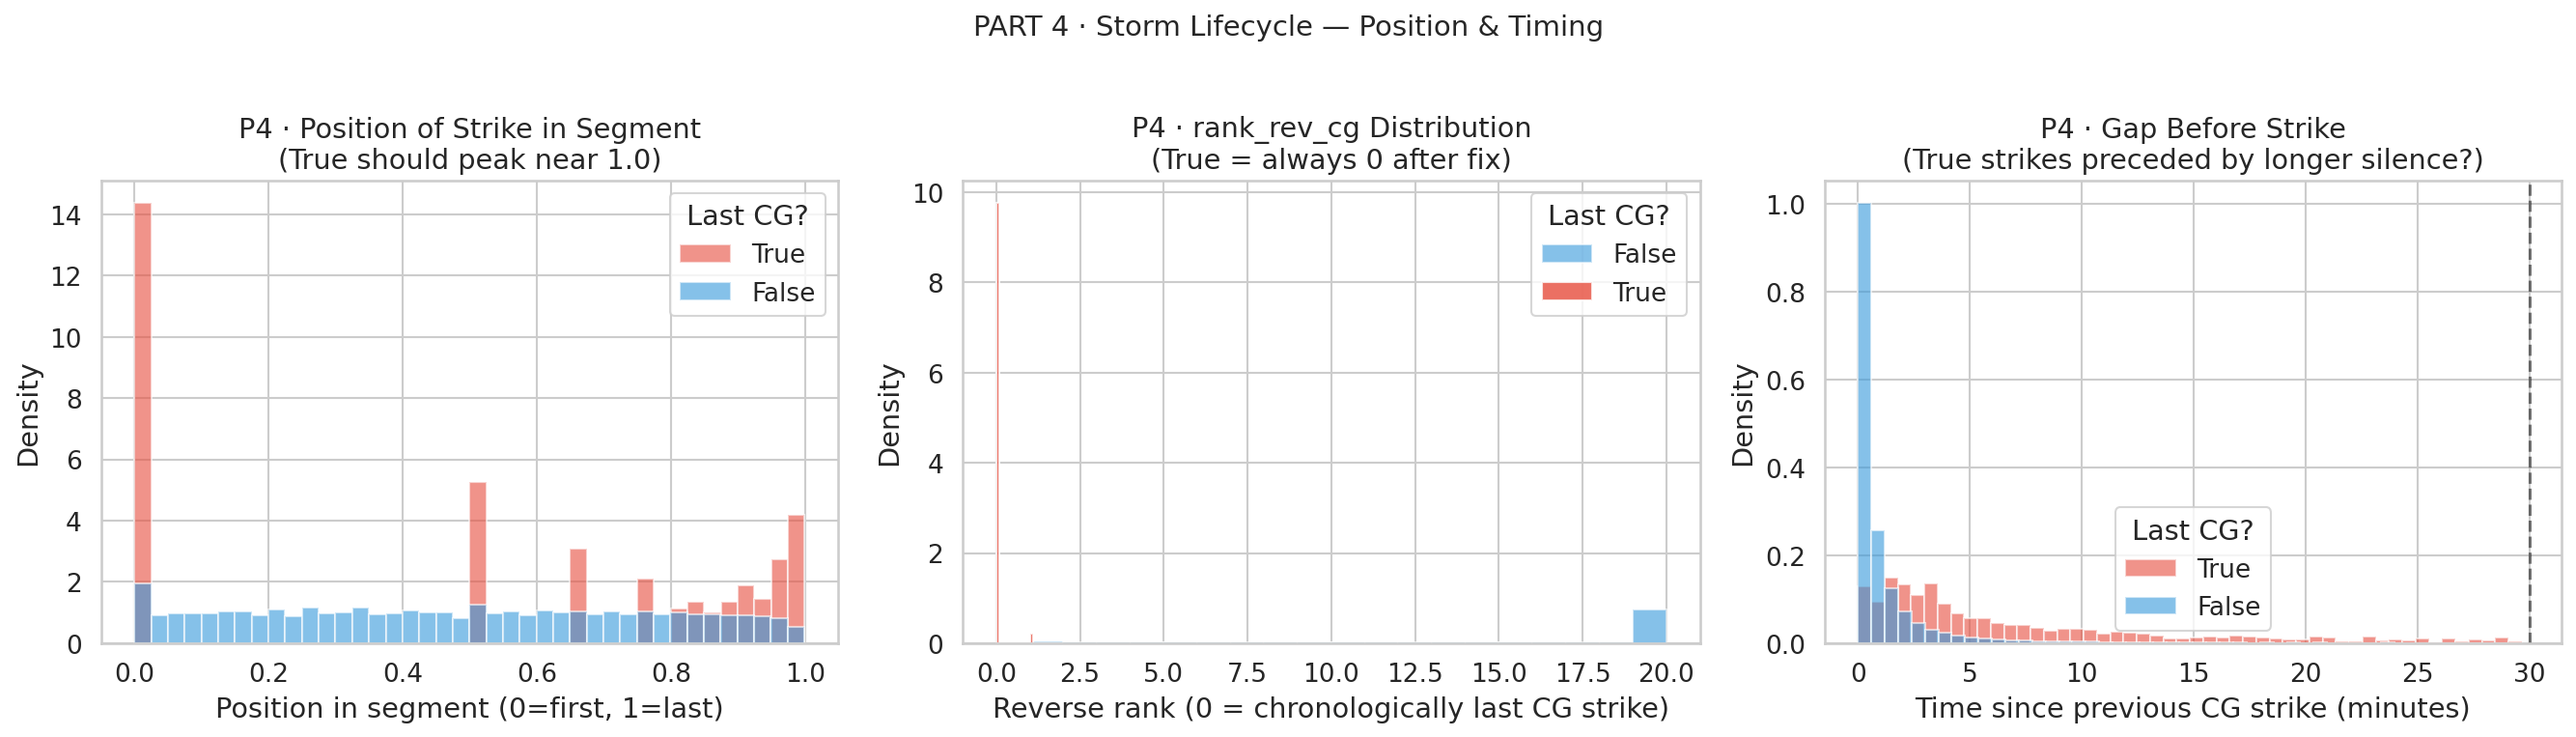
\includegraphics[width=\textwidth]{figures/p4_storm_lifecycle_timing.png}
  \caption{Storm lifecycle timing patterns across all 2,627 segments}
  \label{fig:lifecycle_timing}
\end{figure}

The following physical mechanism drives predictability:
\begin{itemize}[leftmargin=1.5em]
  \item As electrical charge depletes, CG strike frequency drops
  \item Remaining charge tends to produce positive-polarity strikes
  \item The storm cell drifts away as the convective core weakens
  \item Outer-ring (20--50 km) activity collapses as the storm fully dissipates
\end{itemize}

% ============================================================
\section{Airport Profiles}
% ============================================================

\begin{table}[H]
\centering
\caption{Per-airport storm statistics}
\resizebox{\textwidth}{!}{%
\begin{tabular}{lrrrrr}
\toprule
\textbf{Airport} & \textbf{Segments} & \textbf{Median strikes} &
\textbf{Mean strikes} & \textbf{Median dur.\ (min)} & \textbf{Max dur.\ (min)} \\
\midrule
Ajaccio   & 530 & 2.0 & 20.1 &  8.4 & 400.1 \\
Bastia    & 532 & 3.0 & 25.8 & 10.1 & 497.8 \\
Biarritz  & 590 & 3.0 & 16.8 &  7.1 & 387.6 \\
Nantes    & 206 & 2.0 & 21.3 &  8.8 & 381.5 \\
Pise      & 769 & 3.0 & 23.3 & 11.3 & 578.7 \\
\bottomrule
\end{tabular}}
\end{table}

\begin{figure}[H]
  \centering
  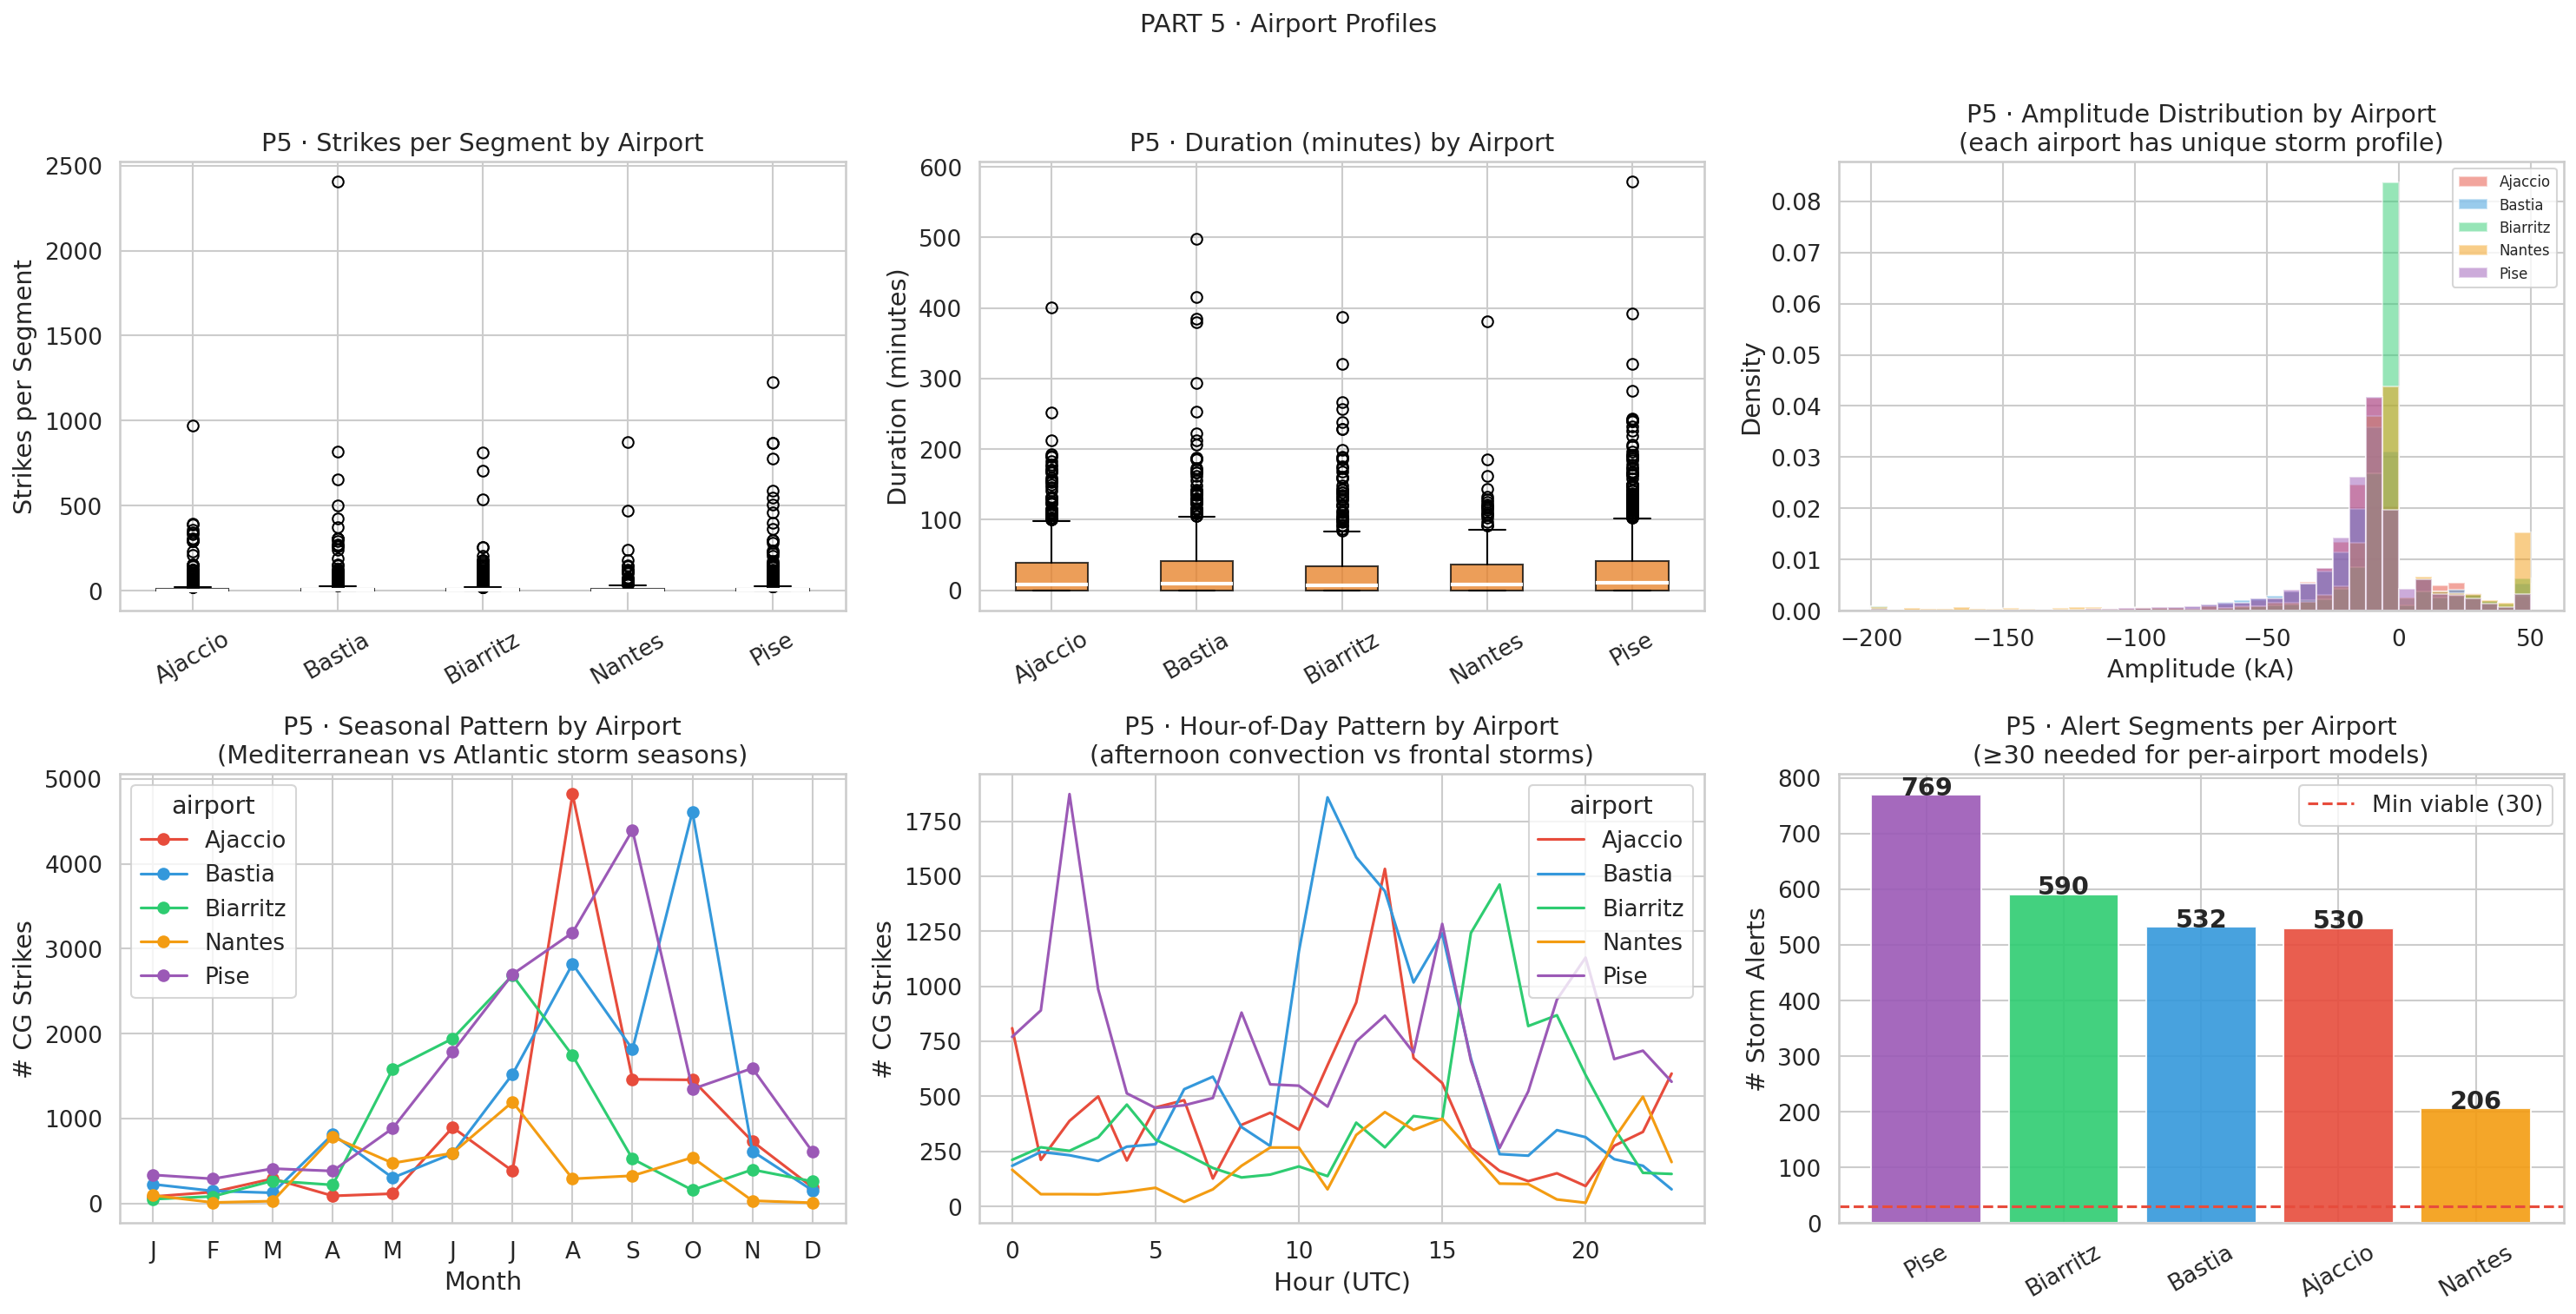
\includegraphics[width=\textwidth]{figures/p5_airport_profiles.png}
  \caption{Per-airport storm segment profiles}
  \label{fig:airports}
\end{figure}

\noindent \textbf{Key observations}:
\begin{itemize}[leftmargin=1.5em]
  \item Pise is the largest airport (769 segments) with the longest storms (median 11.3 min)
  \item Biarritz has the shortest storms (median 7.1 min) — quick-onset maritime convection
  \item Bastia has the highest mean strike count per segment (25.8) — intense Corsican storms
  \item All airports show extreme outliers (storms $>$6 hours)
  \item Nantes is under-represented (206 segments) — potential leave-one-airport-out risk
\end{itemize}

Airport differences are moderate and captured by target encoding (\texttt{airport\_target\_enc}).

\begin{figure}[H]
  \centering
  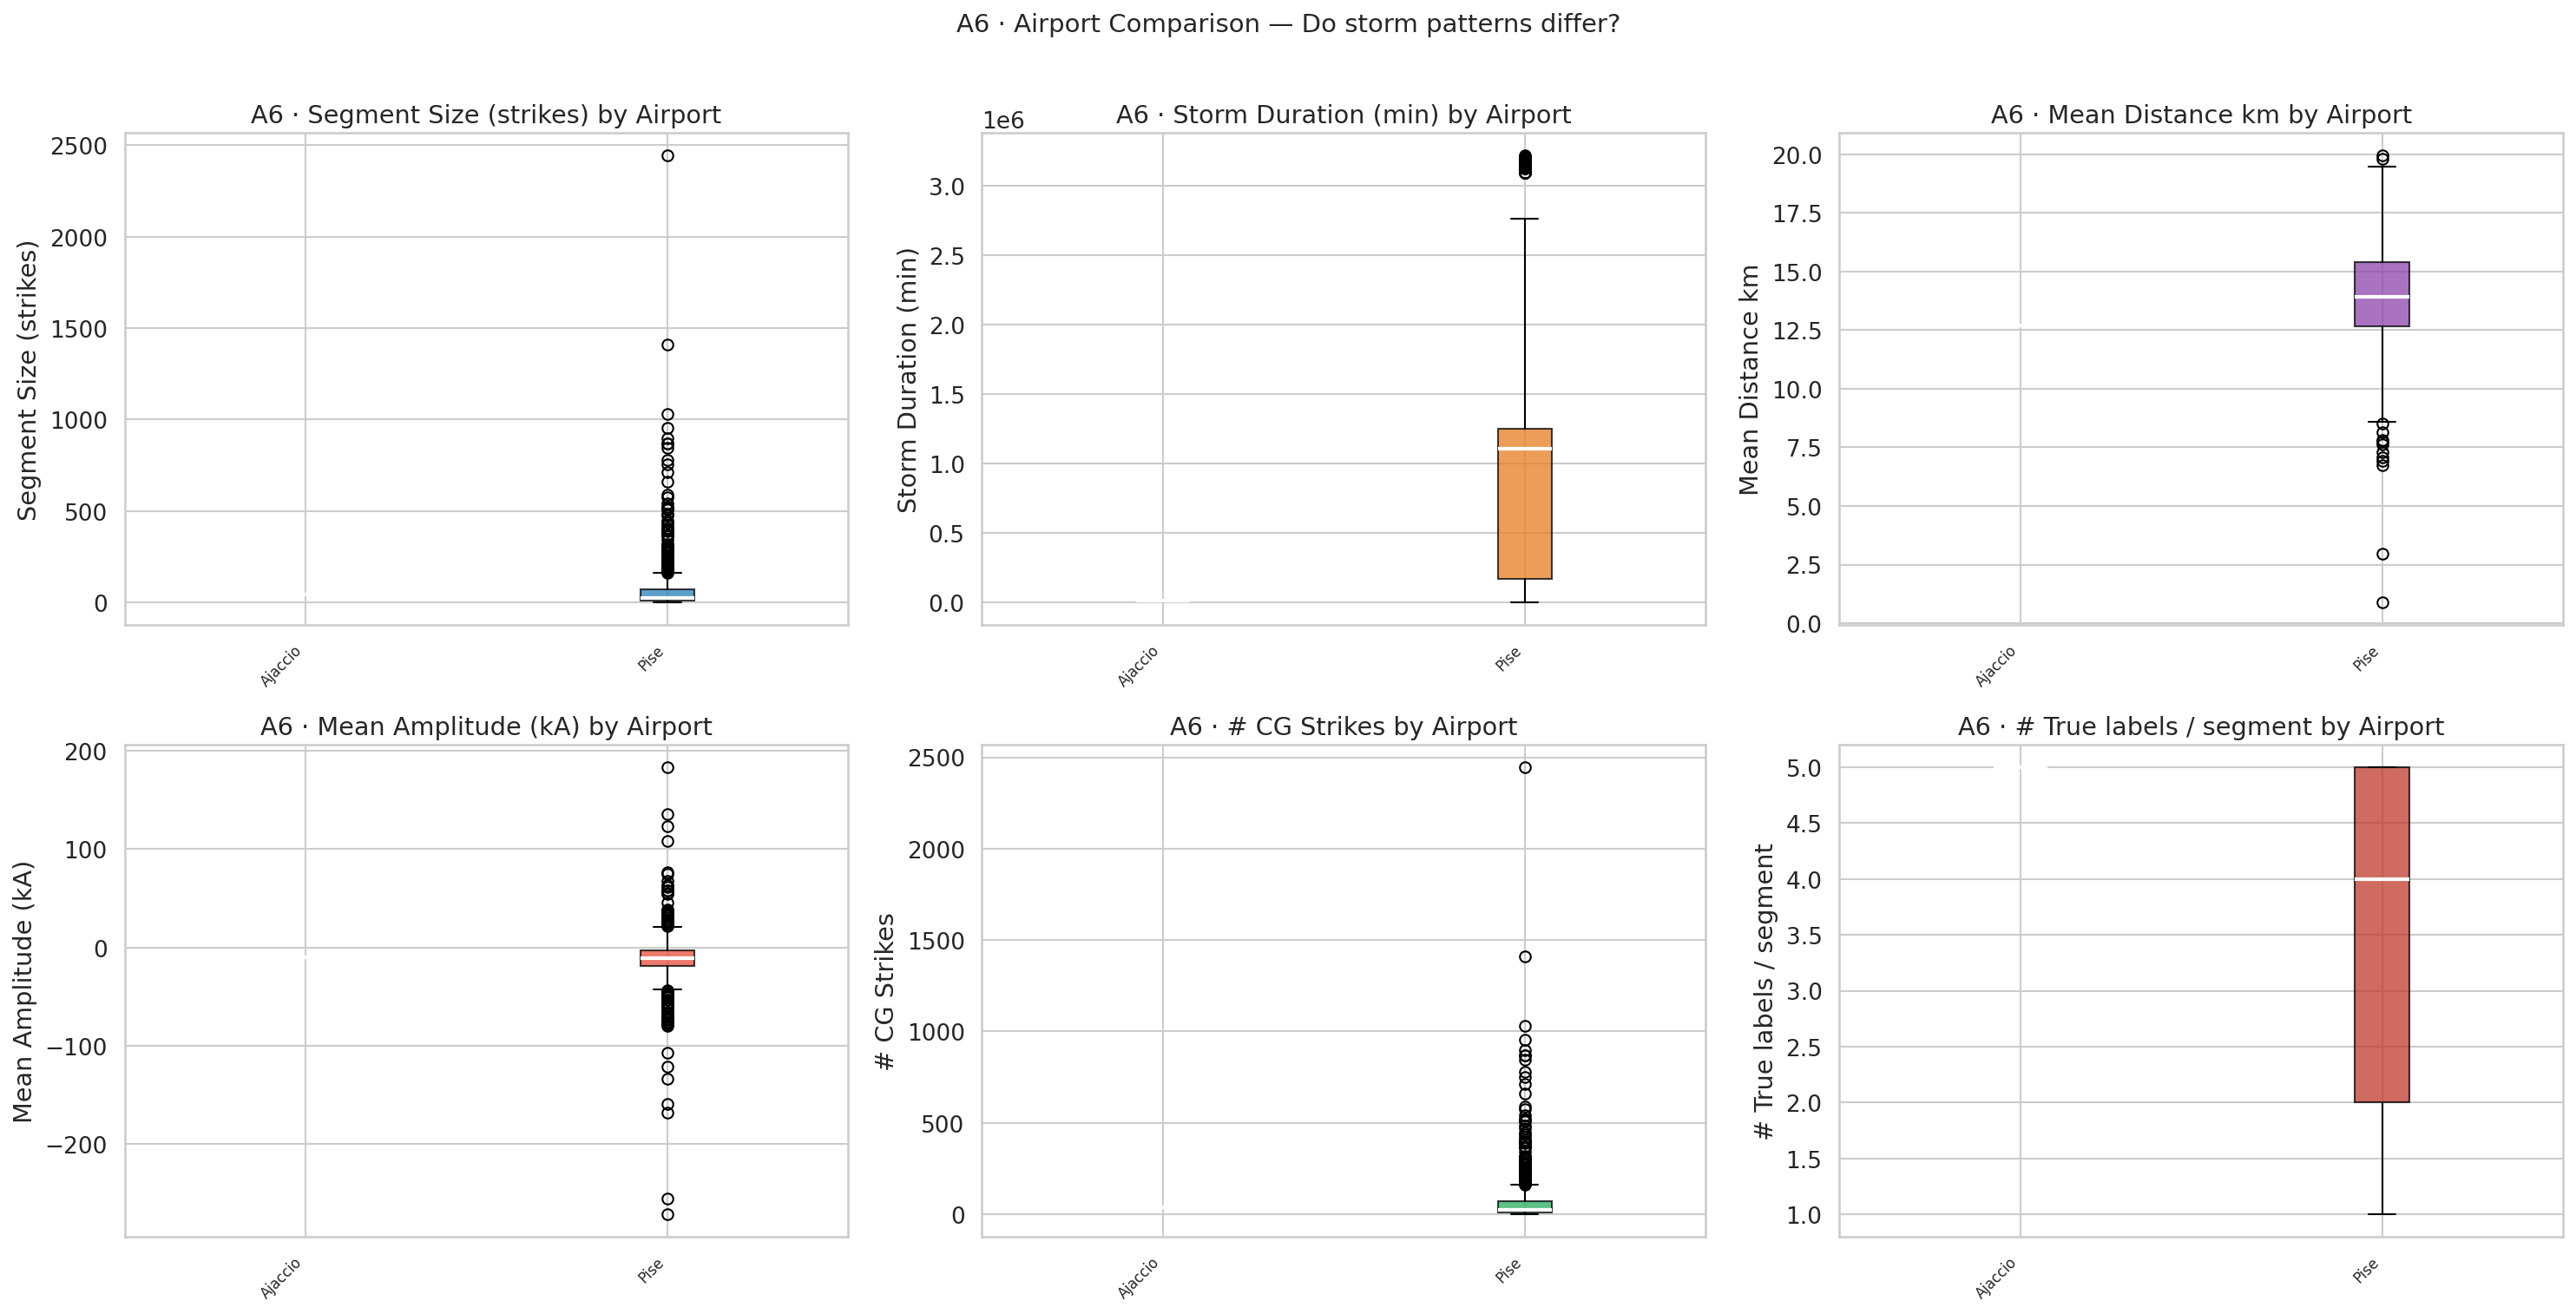
\includegraphics[width=\textwidth]{figures/axis6_per_airport_boxplots.png}
  \caption{Feature distributions per airport}
  \label{fig:airport_boxes}
\end{figure}

% ============================================================
\section{Feature Engineering}
% ============================================================

\subsection{Overview}

41 features are engineered across 11 groups. Each group targets a distinct
physical aspect of storm decay. Table~\ref{tab:features_overview} summarises all groups.

\begin{table}[H]
\centering
\caption{Feature groups overview}
\label{tab:features_overview}
\begin{tabular}{clrc}
\toprule
\textbf{Group} & \textbf{Name} & \textbf{Features} & \textbf{Signal strength} \\
\midrule
A & Amplitude decomposition  & 3 & High \\
B & Segment context          & 6 & High \\
C & Position within segment  & 3 & Moderate \\
D & Temporal dynamics        & 8 & Very High \\
E & Rolling window activity  & 5 & High \\
F & Silence thresholds       & 3 & High \\
G & Interaction features     & 2 & Moderate \\
H & Outer ring context       & 1 & High \\
I & Calendar features        & 4 & Low \\
J & Raw physical             & 5 & Low--Moderate \\
K & Airport encoding         & 1 & Moderate \\
\midrule
  & \textbf{Total}           & \textbf{41} & \\
\bottomrule
\end{tabular}
\end{table}

\subsection{Group A — Amplitude Decomposition}

\begin{itemize}[leftmargin=1.5em]
  \item \texttt{amplitude}: raw kA value with sign. Negative = normal mature storm.
        Positive = decay indicator.
  \item \texttt{amp\_magnitude}: $|\text{amplitude}|$ — storm intensity regardless of polarity.
        True strikes have 45\% higher magnitude on average.
  \item \texttt{amp\_is\_positive}: binary flag (1 if positive CG) — clean decay indicator
\end{itemize}

\subsection{Group B — Segment Context}

Aggregated statistics over the entire segment, giving each strike awareness of the
storm it belongs to:
\texttt{seg\_size\_cg}, \texttt{seg\_mean\_amp}, \texttt{seg\_std\_amp},
\texttt{seg\_duration\_min} ($|r|=0.215$, second strongest feature),
\texttt{seg\_mean\_dist}, \texttt{seg\_pos\_cg\_ratio}.

\subsection{Group C — Position Within Segment}

\begin{itemize}[leftmargin=1.5em]
  \item \texttt{rank\_in\_seg}: chronological index (0 = first strike)
  \item \texttt{pct\_position}: normalised position in $[0,1]$, where 1.0 = last strike.
        True labels are concentrated near 1.0.
  \item \texttt{rank\_rev\_cg}: reverse rank (0 = last strike). Always 0 for True labels.
\end{itemize}

\subsection{Group D — Temporal Dynamics}

\begin{itemize}[leftmargin=1.5em]
  \item \texttt{time\_since\_prev}: \textbf{strongest single feature} ($|r|=0.216$).
        Growing silence signals storm ending.
  \item \texttt{dist\_delta}: distance change from previous strike.
        Positive = storm moving away = ending signal.
  \item \texttt{amp\_delta}: amplitude change — weakening storm trend.
  \item \texttt{storm\_speed}: displacement magnitude per minute.
\end{itemize}

\noindent\textbf{Additional temporal features from lifecycle analysis:}

\begin{itemize}[leftmargin=1.5em]
  \item \texttt{time\_since\_first\_strike}: minutes elapsed since the alert opened.
        Captures absolute storm age — older storms are more likely to be ending.
  \item \texttt{interarrival\_mean\_last5}: mean gap (in minutes) between the last 5 CG strikes.
        Lengthening inter-arrival time is a key decay signal.
  \item \texttt{interarrival\_std\_last5}: standard deviation of the last 5 inter-arrival gaps.
        High variability in recent gaps indicates an irregular, weakening storm rhythm.
  \item \texttt{centroid\_shift}: distance (km) the strike centroid has moved within the segment.
        A drifting centroid confirms the storm cell is translating away from the airport.
\end{itemize}

\subsection{Group E — Rolling Window Activity}

Activity in the last $N$ minutes before each strike, computed using a time-indexed
rolling window within each segment:

\begin{itemize}[leftmargin=1.5em]
  \item \texttt{cg\_count\_5min}, \texttt{cg\_count\_10min}, \texttt{cg\_count\_30min}:
        declining counts signal storm decay ($|r| \approx 0.16$).
        Note: 5min/10min/30min are highly correlated ($r=0.97$). LightGBM handles this.
  \item \texttt{rolling\_mean\_mag\_10min}: magnitude trend over 10 min.
  \item \texttt{rolling\_pos\_ratio\_10min}: fraction of recent strikes that are
        positive-polarity ($|r|=0.107$).
\end{itemize}

\subsection{Group F — Silence Threshold Features}

Binary flags encoding regime transitions:

\begin{table}[H]
\centering
\caption{Silence threshold features and their signal strength}
\begin{tabular}{lrl}
\toprule
\textbf{Feature} & $|r|$ & \textbf{Interpretation} \\
\midrule
\texttt{silence\_over\_10min} & 0.174 & Any 10-min gap is a strong ending signal \\
\texttt{silence\_over\_15min} & 0.144 & Stronger threshold \\
\texttt{silence\_over\_20min} & 0.108 & $>$20 min silence = storm nearly ended \\
\bottomrule
\end{tabular}
\end{table}

\subsection{Group G — Interaction Features}

\begin{itemize}[leftmargin=1.5em]
  \item \texttt{silence\_x\_dist\_away}: (silence $>$ 15 min) AND (storm moving away).
        Captures the joint condition where both decay signals are active simultaneously.
        $|r|=0.109$.
  \item \texttt{weak\_and\_moving\_away}: (amplitude below segment mean) AND (moving away).
\end{itemize}

\subsection{Group H — Outer Ring Context}

The most novel feature: CG strike count in the 20--50 km ring around the airport
in the last 10 minutes. Computed from the 450K outside-zone rows.

\begin{table}[H]
\centering
\caption{Outer ring activity by class}
\begin{tabular}{lrr}
\toprule
\textbf{Class} & \textbf{Mean outer ring count} & \textbf{Std} \\
\midrule
\textcolor{falsecolor}{\textbf{False}} & 22.5 & 31.1 \\
\textcolor{truecolor}{\textbf{True}}   & 2.4  & 7.5  \\
\midrule
Ratio & \textbf{8.8$\times$ lower} & \\
\bottomrule
\end{tabular}
\end{table}

\noindent When the surrounding storm system collapses, the last strike is imminent.
This feature has $|r|=0.138$ and is largely independent of all other features.

\subsection{Groups I--K — Calendar, Raw Physical, Airport Encoding}

Calendar features (\texttt{hour}, \texttt{month}, \texttt{is\_summer}, \texttt{is\_afternoon})
provide weak seasonal context ($|r| \approx 0.03$--$0.05$). Raw physical features
(\texttt{maxis}, \texttt{dist}, \texttt{azimuth}, \texttt{strike\_x/y}) are included
as base signal. Airport target encoding (\texttt{airport\_target\_enc}) encodes the
per-airport baseline True rate.

% ============================================================
\section{Feature Signal Strength Ranking}
% ============================================================

\begin{table}[H]
\centering
\caption{Top 20 features by point-biserial correlation with target}
\begin{tabular}{rlrll}
\toprule
\textbf{Rank} & \textbf{Feature} & $|r|$ & \textbf{Group} & \textbf{Signal type} \\
\midrule
1  & \texttt{time\_since\_prev}       & 0.216 & D & Silence duration \\
2  & \texttt{seg\_duration\_min}      & 0.215 & B & Segment context \\
3  & \texttt{silence\_over\_10min}    & 0.174 & F & Regime threshold \\
4  & \texttt{cg\_count\_5min}         & 0.161 & E & Rolling activity \\
5  & \texttt{cg\_count\_10min}        & 0.161 & E & Rolling activity \\
6  & \texttt{cg\_count\_30min}        & 0.157 & E & Rolling activity \\
7  & \texttt{silence\_over\_15min}    & 0.144 & F & Regime threshold \\
8  & \texttt{seg\_size\_cg}           & 0.143 & B & Segment context \\
9  & \texttt{outer\_ring\_cg\_10min}  & 0.138 & H & Outer ring context \\
10 & \texttt{seg\_pos\_cg\_ratio}     & 0.127 & B & Polarity in segment \\
11 & \texttt{rank\_rev\_cg}           & 0.124 & C & Position \\
12 & \texttt{rank\_in\_seg}           & 0.110 & C & Position \\
13 & \texttt{storm\_speed}            & 0.110 & D & Motion \\
14 & \texttt{silence\_x\_dist\_away}  & 0.109 & G & Interaction \\
15 & \texttt{silence\_over\_20min}    & 0.108 & F & Regime threshold \\
16 & \texttt{rolling\_pos\_ratio\_10min} & 0.107 & E & Rolling polarity \\
17 & \texttt{seg\_mean\_dist}         & 0.097 & B & Segment context \\
18 & \texttt{seg\_mean\_mag}          & 0.094 & B & Amplitude context \\
19 & \texttt{rolling\_mean\_mag\_10min}  & 0.087 & E & Rolling magnitude \\
20 & \texttt{rolling\_mean\_dist\_10min} & 0.074 & E & Rolling distance \\
\bottomrule
\end{tabular}
\end{table}

\begin{figure}[H]
  \centering
  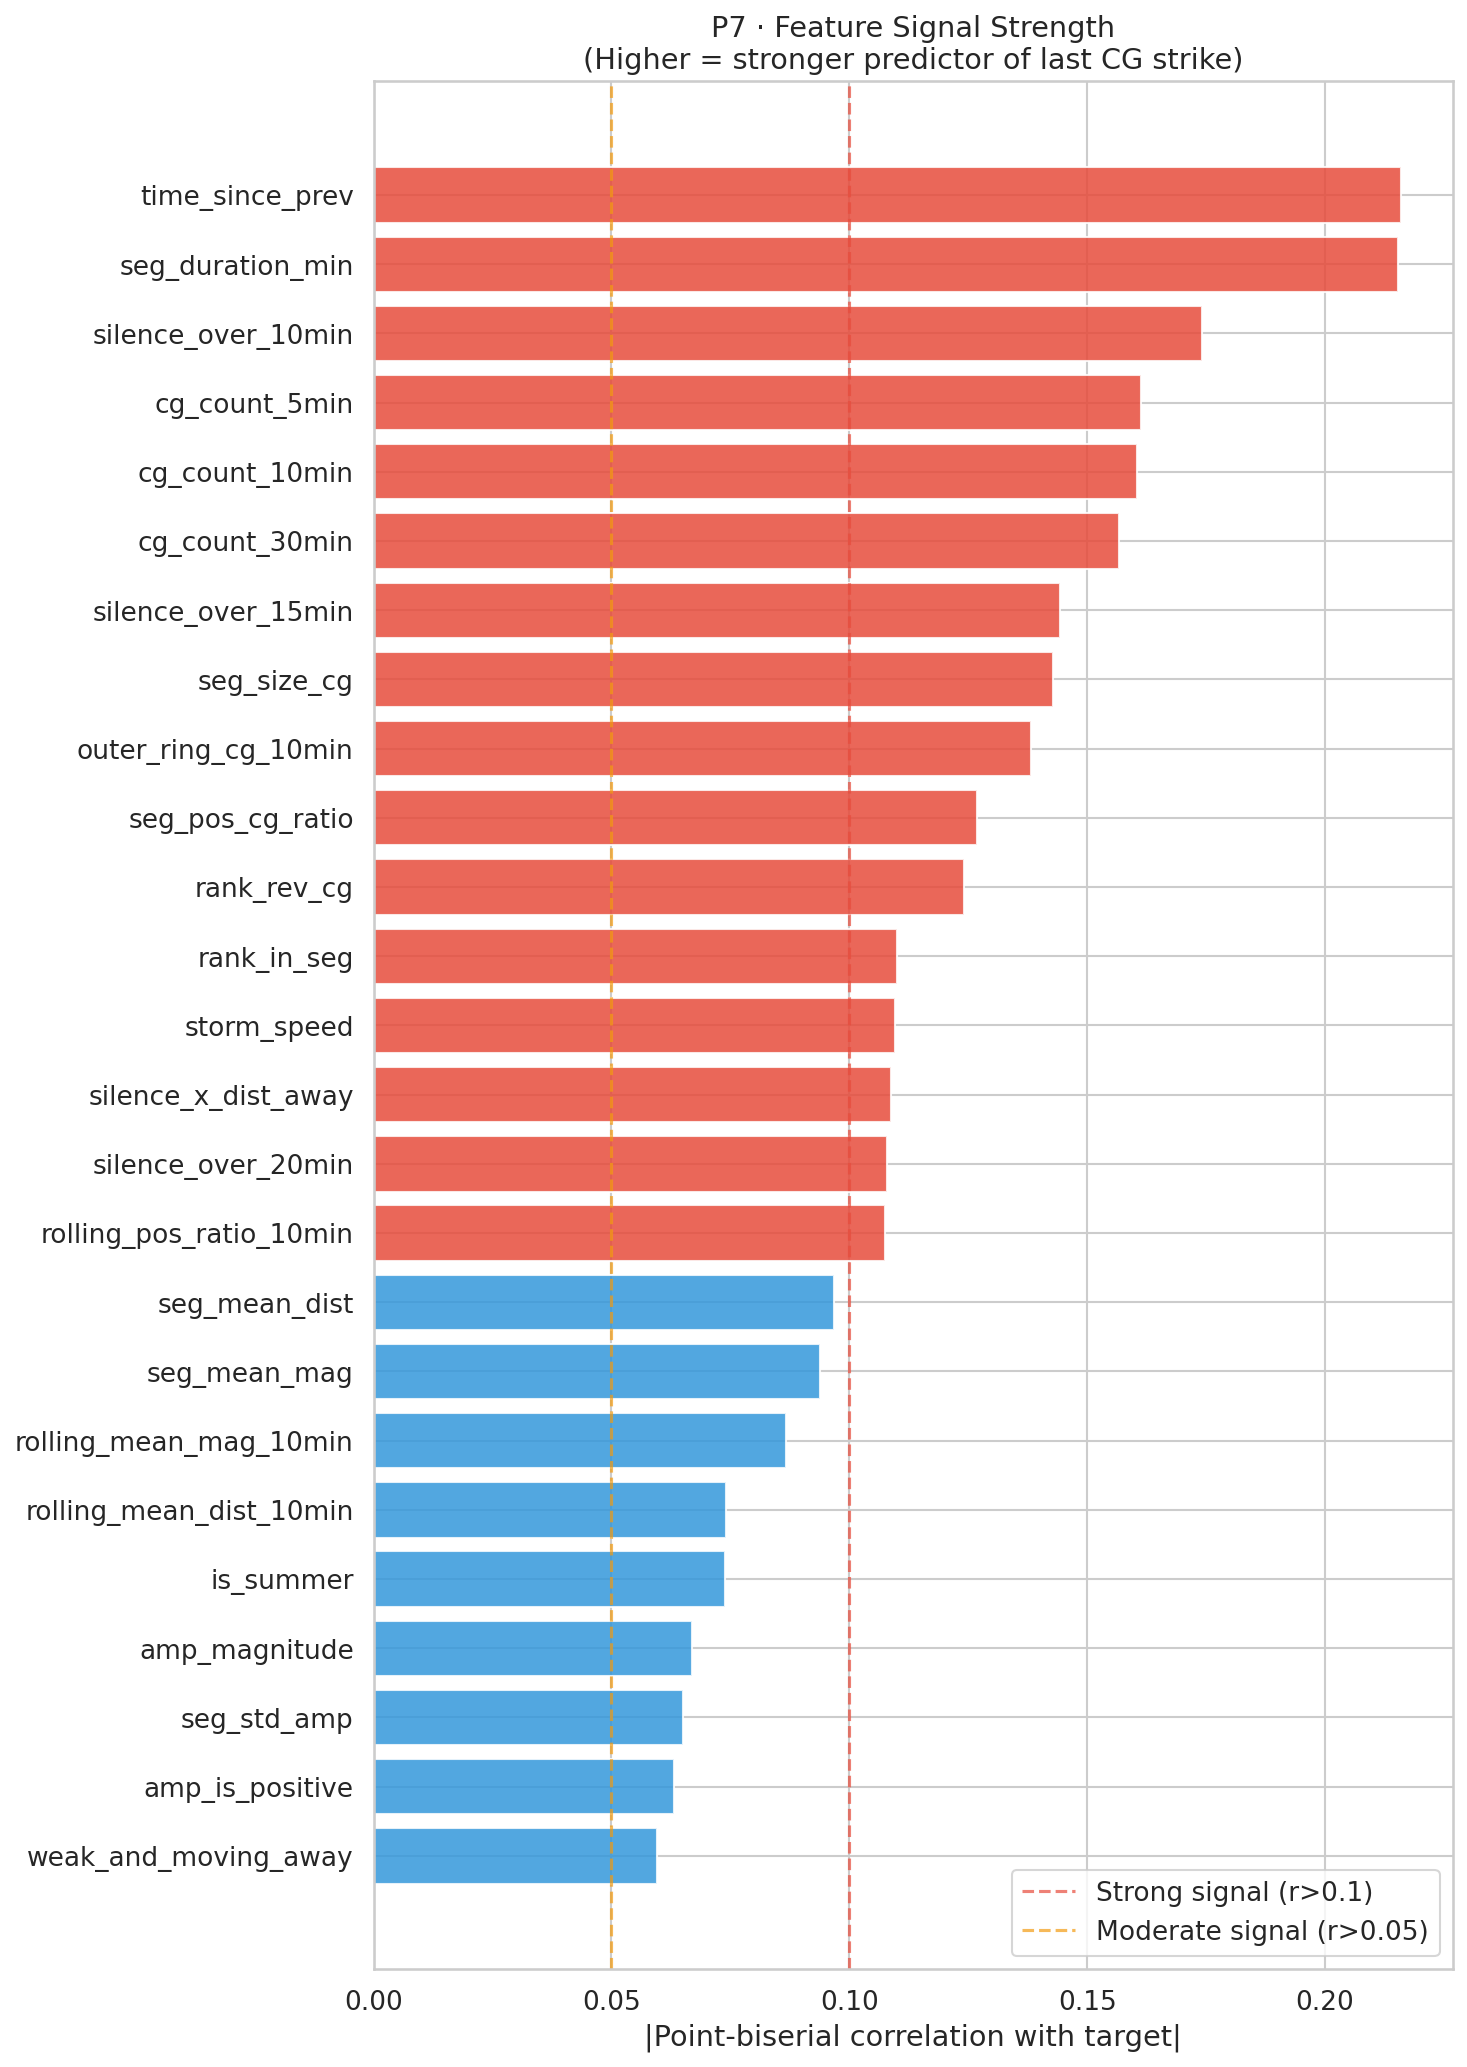
\includegraphics[width=\textwidth]{figures/p7_feature_signal_strength.png}
  \caption{Feature signal strength — point-biserial correlation with target}
  \label{fig:signal}
\end{figure}

% ============================================================
\section{Feature Correlation and Redundancy}
% ============================================================

\begin{figure}[H]
  \centering
  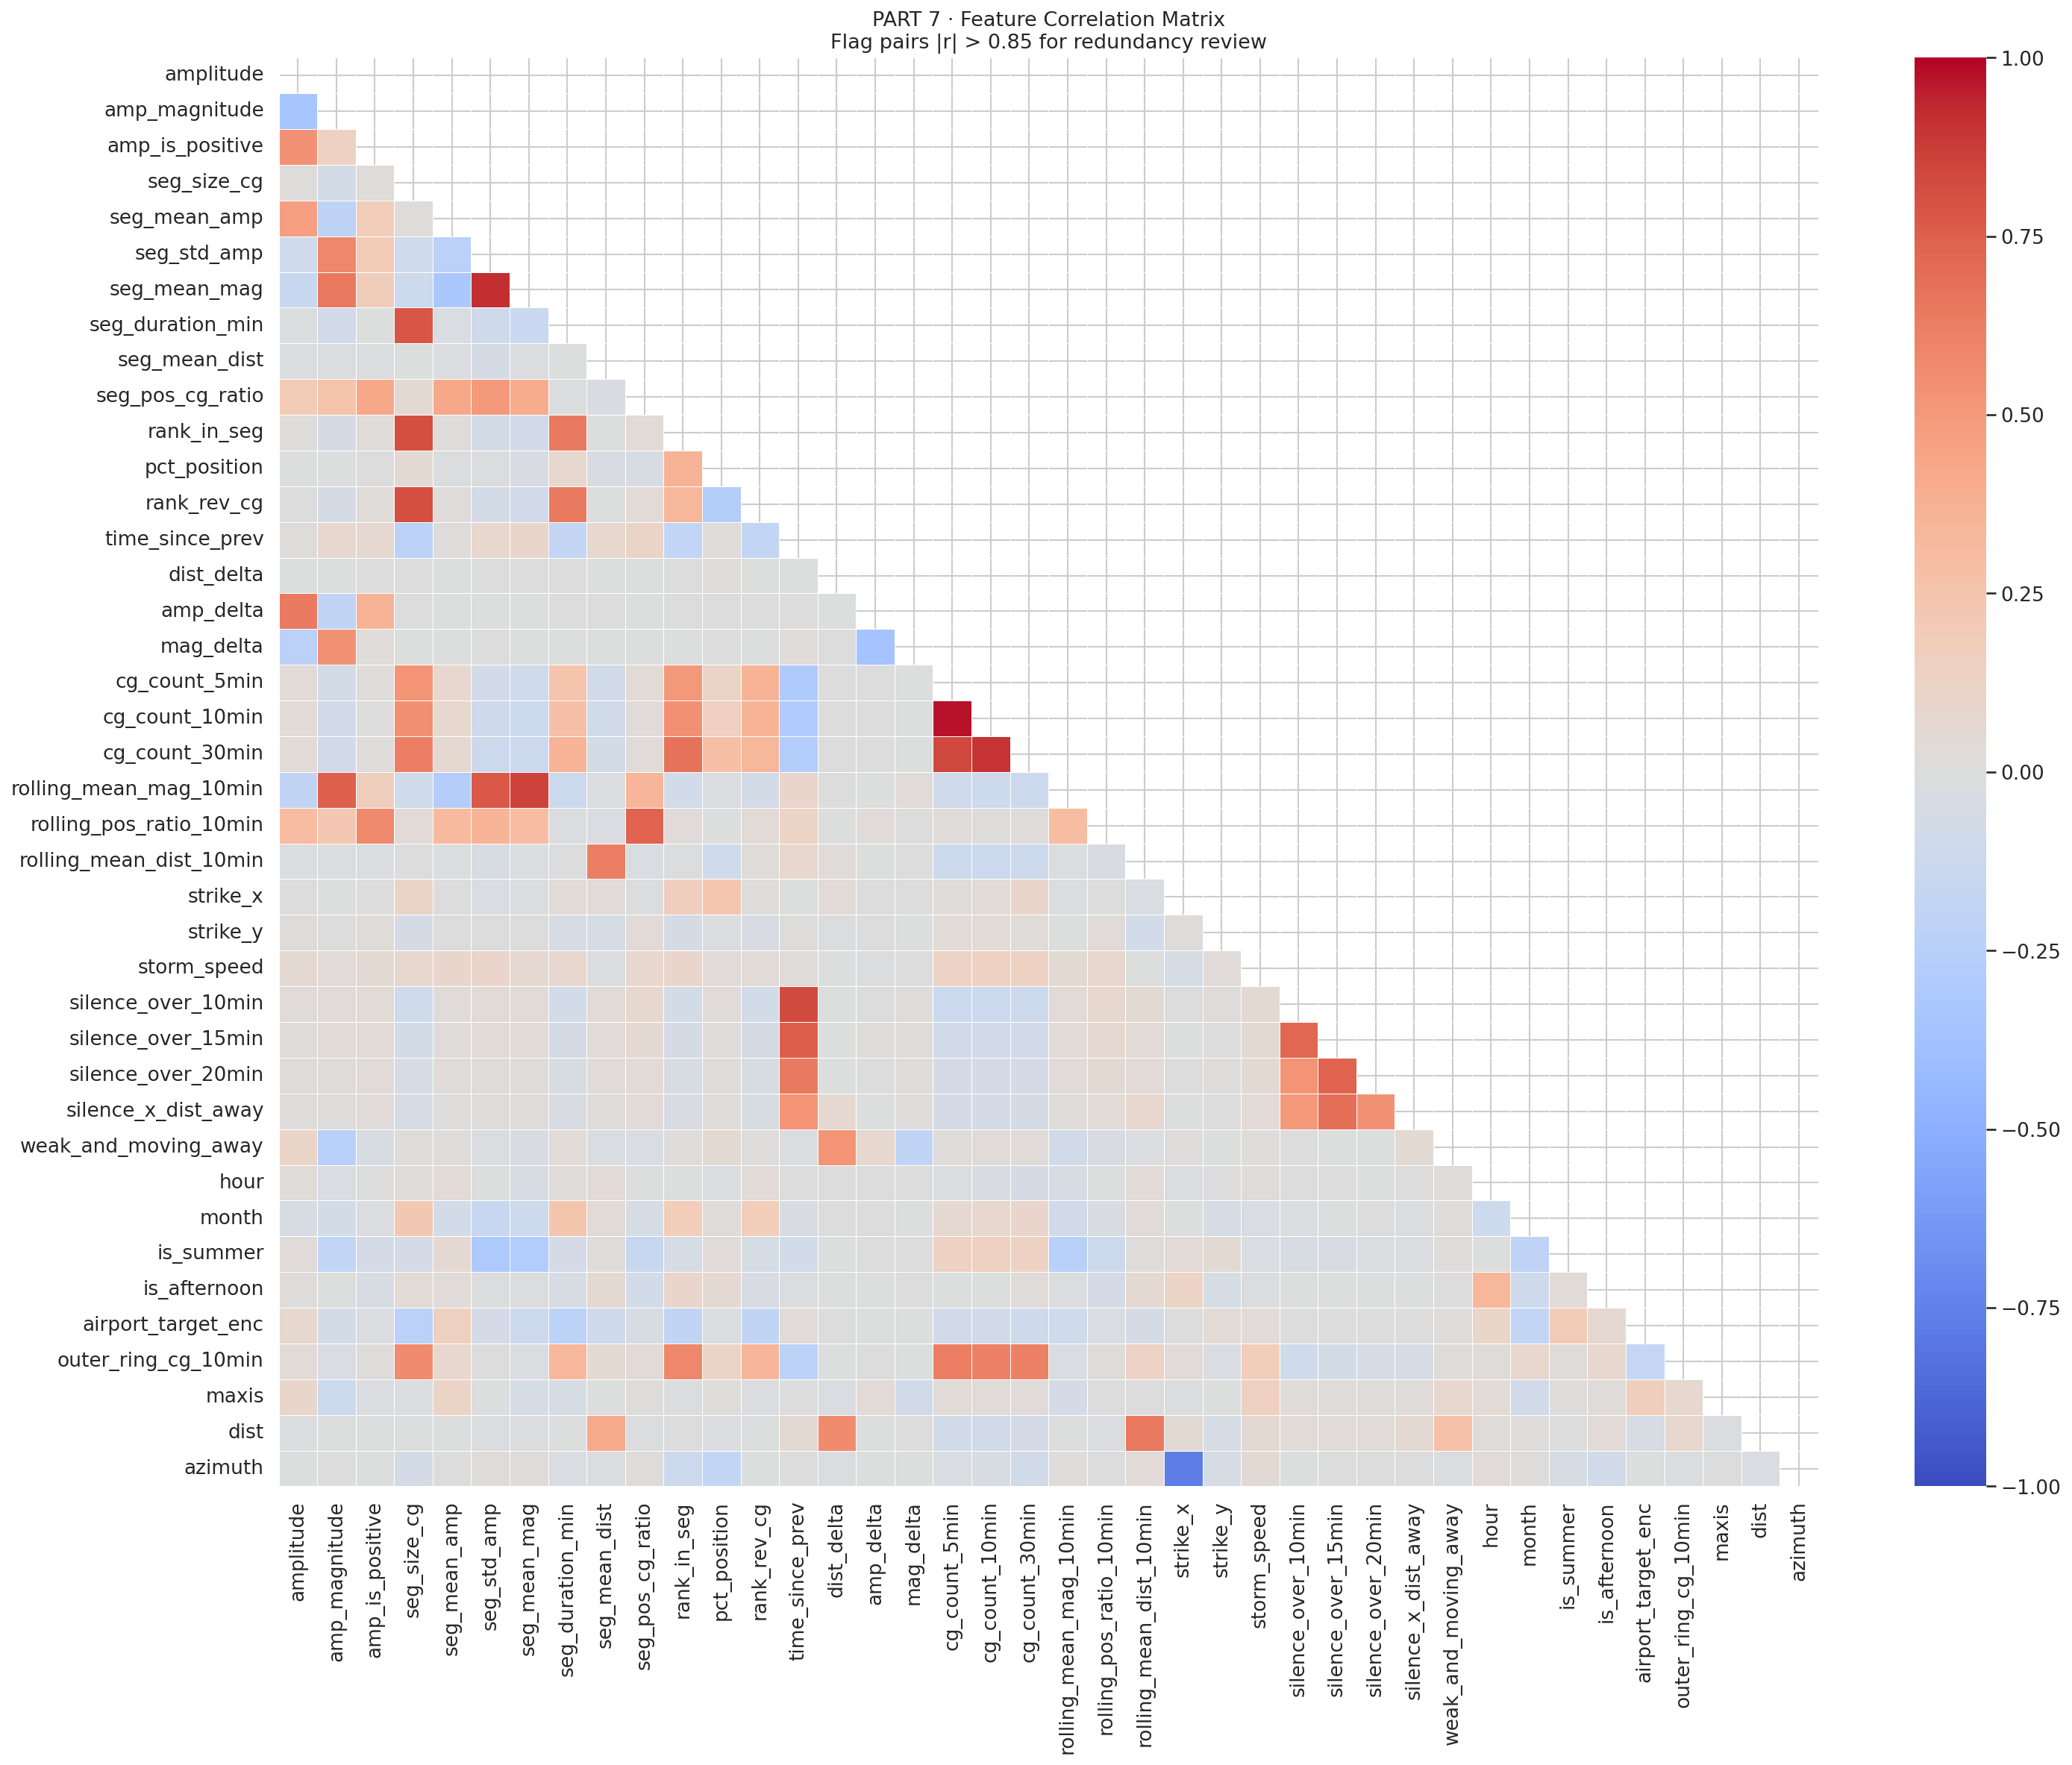
\includegraphics[width=\textwidth]{figures/p7_correlation_matrix.png}
  \caption{Feature correlation matrix}
  \label{fig:corr}
\end{figure}

\subsection*{High-Correlation Pairs ($|r| > 0.85$)}

\begin{table}[H]
\centering
\caption{Redundant feature pairs}
\begin{tabular}{llrl}
\toprule
\textbf{Feature A} & \textbf{Feature B} & $r$ & \textbf{Action} \\
\midrule
\texttt{cg\_count\_5min} & \texttt{cg\_count\_10min} & +0.974 & Keep both (different time scales) \\
\texttt{seg\_std\_amp}   & \texttt{seg\_mean\_mag}   & +0.921 & Keep both (different statistics) \\
\texttt{cg\_count\_10min} & \texttt{cg\_count\_30min} & +0.903 & Keep all three \\
\texttt{seg\_mean\_mag}  & \texttt{rolling\_mean\_mag\_10min} & +0.857 & Keep both \\
\bottomrule
\end{tabular}
\end{table}

\noindent Despite high pairwise correlations within the rolling count group, all features
are retained. Gradient boosting (LightGBM) handles multicollinearity well and the different
time scales (5, 10, 30 min) may interact differently with other features at split decisions.

% ============================================================
\section{What Works and What Does Not}
% ============================================================

\subsection{Strong Strategic Moves}

\begin{enumerate}[leftmargin=1.5em]
  \item \textbf{Time gap (silence) as primary feature}: The gap before a strike is the
        single most informative feature. Growing silence = storm ending. Model this both
        continuously (\texttt{time\_since\_prev}) and as threshold dummies (\texttt{silence\_over\_N}).

  \item \textbf{Outer ring collapse}: Monitoring the 20--50 km surrounding area is novel
        and independent. The 8.8$\times$ activity drop before the last strike is dramatic
        and not captured by any within-zone feature.

  \item \textbf{Amplitude polarity}: Positive-polarity CG strikes increase near storm end.
        Modelled at three granularities: raw value, binary flag, rolling ratio.

  \item \textbf{Segment-level context}: Each strike's probability depends on the storm it
        belongs to. Segment duration, size, and mean polarity are strong context features
        ($|r| \approx 0.14$--$0.22$).

  \item \textbf{Interaction feature}: Combining silence $>$15 min AND moving away captures
        the joint end condition more precisely than either signal alone.

  \item \textbf{GroupKFold by segment}: Using segment identity as the CV fold prevents
        data leakage from the same storm appearing in both train and validation.
\end{enumerate}

\subsection{What Does Not Work}

\begin{table}[H]
\centering
\caption{Features with weak or no signal}
\begin{tabular}{lp{9cm}}
\toprule
\textbf{Feature} & \textbf{Finding} \\
\midrule
\texttt{azimuth}           & No directional effect. Storms approach from all directions
                             equally — isotropic distribution confirmed. \\
Calendar features          & Hour, month, season signals are too weak ($|r| < 0.05$)
                             at strike level. Useful only as soft regularisation. \\
\texttt{strike\_x/y}       & Geographic coordinates are less useful than derived
                             \texttt{dist} and \texttt{azimuth}. \\
\texttt{maxis} (raw)       & Flash energy is only weakly correlated with last-strike
                             probability. Included but low priority. \\
Rolling distance trend     & \texttt{rolling\_mean\_dist\_10min} is the weakest
                             rolling feature ($|r|=0.074$). \\
\bottomrule
\end{tabular}
\end{table}

% ============================================================
\section{Final Feature List for Model Training}
% ============================================================

\begin{table}[H]
\centering
\caption{Complete feature list (41 features)}
\begin{tabular}{llll}
\toprule
\textbf{Feature} & \textbf{Group} & \textbf{Type} & \textbf{Priority} \\
\midrule
\texttt{amplitude}                & A & continuous & High \\
\texttt{amp\_magnitude}           & A & continuous & High \\
\texttt{amp\_is\_positive}        & A & binary     & High \\
\texttt{seg\_size\_cg}            & B & continuous & High \\
\texttt{seg\_mean\_amp}           & B & continuous & Medium \\
\texttt{seg\_std\_amp}            & B & continuous & Medium \\
\texttt{seg\_duration\_min}       & B & continuous & High \\
\texttt{seg\_mean\_dist}          & B & continuous & Medium \\
\texttt{seg\_pos\_cg\_ratio}      & B & continuous & High \\
\texttt{rank\_in\_seg}            & C & continuous & Medium \\
\texttt{pct\_position}            & C & continuous & Medium \\
\texttt{rank\_rev\_cg}            & C & continuous & Medium \\
\texttt{time\_since\_prev}           & D & continuous & \textbf{Very High} \\
\texttt{dist\_delta}               & D & continuous & Medium \\
\texttt{amp\_delta}                & D & continuous & Medium \\
\texttt{storm\_speed}              & D & continuous & Medium \\
\texttt{time\_since\_first\_strike} & D & continuous & Medium \\
\texttt{interarrival\_mean\_last5}  & D & continuous & High \\
\texttt{interarrival\_std\_last5}   & D & continuous & Medium \\
\texttt{centroid\_shift}            & D & continuous & Medium \\
\texttt{cg\_count\_5min}          & E & continuous & High \\
\texttt{cg\_count\_10min}         & E & continuous & High \\
\texttt{cg\_count\_30min}         & E & continuous & High \\
\texttt{rolling\_mean\_mag\_10min}  & E & continuous & Medium \\
\texttt{rolling\_pos\_ratio\_10min} & E & continuous & Medium \\
\texttt{rolling\_mean\_dist\_10min} & E & continuous & Low \\
\texttt{silence\_over\_10min}     & F & binary     & High \\
\texttt{silence\_over\_15min}     & F & binary     & High \\
\texttt{silence\_over\_20min}     & F & binary     & High \\
\texttt{silence\_x\_dist\_away}   & G & binary     & Medium \\
\texttt{weak\_and\_moving\_away}  & G & binary     & Medium \\
\texttt{outer\_ring\_cg\_10min}   & H & continuous & High \\
\texttt{hour}                     & I & categorical & Low \\
\texttt{month}                    & I & categorical & Low \\
\texttt{is\_summer}               & I & binary     & Low \\
\texttt{is\_afternoon}            & I & binary     & Low \\
\texttt{maxis}                    & J & continuous & Low \\
\texttt{dist}                     & J & continuous & Medium \\
\texttt{azimuth}                  & J & continuous & Very Low \\
\texttt{strike\_x}                & J & continuous & Low \\
\texttt{strike\_y}                & J & continuous & Low \\
\texttt{airport\_target\_enc}     & K & continuous & Medium \\
\bottomrule
\end{tabular}
\end{table}

% ============================================================
\section{Model Training Strategy}
% ============================================================

\subsection{Validation Framework}

\begin{enumerate}[leftmargin=1.5em]
  \item \textbf{Primary}: GroupKFold ($k=5$) grouped by \texttt{segment\_key} —
        prevents leakage from the same storm in both train and validation.
  \item \textbf{Secondary}: Temporal split — train on events before 2021,
        validate on 2021+ events.
  \item \textbf{Stress test}: Leave-one-airport-out — tests generalisation to unseen airports.
\end{enumerate}

\subsection{Recommended Model}

\begin{table}[H]
\centering
\caption{Recommended model configuration}
\begin{tabular}{ll}
\toprule
\textbf{Parameter} & \textbf{Value} \\
\midrule
Algorithm              & LightGBM \\
\texttt{scale\_pos\_weight} & 20 (1:20 imbalance) \\
Objective              & \texttt{binary} \\
Primary metric         & F1-score \\
Secondary metrics      & AUC-ROC, Brier Score \\
Decision threshold     & Tuned (not default 0.5) \\
\bottomrule
\end{tabular}
\end{table}

\subsection{Baselines to Beat}

All three rule-baseline metrics must be exceeded simultaneously:

\begin{table}[H]
\centering
\begin{tabular}{lrl}
\toprule
\textbf{Metric} & \textbf{Rule baseline} & \textbf{Target} \\
\midrule
F1-Score    & 0.9885 & $>$ 0.9885 \\
AUC-ROC     & 0.9994 & $>$ 0.9994 \\
Brier Score & 0.0011 & $<$ 0.0011 \\
\bottomrule
\end{tabular}
\caption{Performance baselines}
\end{table}

% ============================================================
\section{Conclusion}
% ============================================================

The EDA reveals a well-structured prediction problem grounded in the physics of
thunderstorm decay. The key predictive signals — growing silence, collapsing outer-ring
activity, and polarity shift toward positive CG — are all physically interpretable
and engineered into 41 model-ready features.

The near-perfect rule baseline (F1 = 0.9885) sets a high bar. The ML model's
competitive advantage will come from combining multiple soft signals simultaneously:
a strike with long preceding silence, in a storm whose outer ring has collapsed,
showing recent positive-polarity trend, is almost certainly the last.

The feature engineering framework is complete and validated. Next step: model
training with LightGBM under GroupKFold cross-validation.


\end{document}
